\section{\gls{bier}: \gls{srt} Analysis}

It is assumed, that the loudness matching part of \gls{bier} (AUTOREF SECTION HERE) is a legit way to provide the same \gls{snr} for both conductors when conducting \gls{bier}.
In order to determine, if under this assumption there is a statistically significant difference in intelligibility between \gls{ac} and \gls{bc}, a paired-sample t-Test is performed.
For this test to be viable, it has to be assumed, that both the \gls{srt} for \gls{ac} and \gls{bc} are normally distributed. Hence the distribution of the difference between the two also has to be normally distributed. 
This can be checked by means of a Lilliefors test.
The Lilliefors test checks the null hypothesis, that the input data is coming from a normally distributed population. 
In the given context, the intrasubject difference between the the \gls{ac} \gls{srt} and the \gls{bc} \gls{srt} (see  is tested.
The population mean and variance are estimated based on the input data. The null hypothesis is rejected or confirmed, based on the discrepancy between the Gaussian \gls{cdf}, that is derived from the estimated mean and variance and the empirical distribution.
This procedure is conveniently implemented in the MATLAB\textsuperscript{\textregistered} function \texttt{lillietest}.
The null hypothesis, that the intrasubject \gls{srt} difference is normally distributed, is not rejected at a \SI{5}{\percent} significance level based on the data at hand.\\



 
\begin{table}[H]
\centering
\caption{Average \gls{srt} of the subjects for \gls{ac} and \gls{bc} obtained with \gls{bier}, values are rounded to one digit after the decimal point for representation in the table, not for the underlying calculations.}
\label{tab:srt}
\begin{tabular}{lrrrrrrrrrr}
Subject     & 1   & 2    & 3    & 4    & 5    & 6    & 7     & 8     & 9    & 10   \\
Avg. \gls{srt}\textsubscript{\gls{ac}} & 2.8 & 1.0  & -2.3 & -3.8 & -7.1 & -2.2 & 11.5  & 0.4   & 11.0 & 4.8  \\
Avg. \gls{srt}\textsubscript{\gls{bc}} & 0.7 & 1.6  & 1.1  & -7.2 & -1.3 & -0.6 & 21.5  & 11.4  & 9.7  & 17.5 \\
\gls{srt}\textsubscript{AC} - \gls{srt}\textsubscript{BC}  & 2.0 & -0.6 & -3.4 & -3.3 & -5.8 & -1.6 & -10.0 & -11.0 & 1.3  & 12.8
\end{tabular}
\end{table}

\begin{figure}[H]
\centering
% This file was created by matlab2tikz.
%
%The latest updates can be retrieved from
%  http://www.mathworks.com/matlabcentral/fileexchange/22022-matlab2tikz-matlab2tikz
%where you can also make suggestions and rate matlab2tikz.
%
\begin{tikzpicture}

\begin{axis}[%
width=120mm, 
height=50mm, 
at={(5mm,5mm)}, 
scale only axis,
xmin=-7.9175,
xmax=22.2175,
xlabel style={font=\color{white!15!black}},
xlabel={Data},
ymin=-1.95996398454005,
ymax=1.95996398454005,
ytick={-3.09023230616781,-2.74778138544499,-2.32634787404084,-2.05374891063182,-1.64485362695147,-1.2815515655446,-0.674489750196082,0,0.674489750196082,1.2815515655446,1.64485362695147,2.05374891063182,2.32634787404084,2.74778138544499,3.09023230616781},
yticklabels={{0.001},{0.003},{0.01},{0.02},{0.05},{0.10},{0.25},{0.50},{0.75},{0.90},{0.95},{0.98},{0.99},{0.997},{0.999}},
ylabel style={font=\color{white!15!black}},
ylabel={Probability},
axis background/.style={fill=white},
title style={font=\bfseries},
title={Normal Probability Plot},
axis x line*=bottom,
axis y line*=left,
xmajorgrids,
ymajorgrids,
legend style={legend cell align=left, align=left, draw=white!15!black}
]


\addplot [color=mycolor1]
  table[row sep=crcr]{%
-2.25	-0.674489750196082\\
4.75	0.674489750196082\\
};
\addlegendentry{\gls{ac}, Gaussian Fit}

\addplot [color=mycolor2, draw=none, mark=*, mark options={solid, mycolor2}]
  table[row sep=crcr]{%
-7.1	-1.64485362695147\\
-3.85	-1.03643338949379\\
-2.25	-0.674489750196082\\
-2.2	-0.385320466407568\\
0.365	-0.125661346855074\\
1.025	0.125661346855074\\
2.75	0.385320466407568\\
4.75	0.674489750196082\\
11	1.03643338949379\\
11.5	1.64485362695147\\
};
\addlegendentry{\gls{ac}, Subject Data}



\addplot [color=mycolor3]
  table[row sep=crcr]{%
-0.603	-0.674489750196082\\
11.35	0.674489750196082\\
};
\addlegendentry{\gls{bc}, Gaussian Fit}

\addplot [color=mycolor4, draw=none, mark=*, mark options={solid, mycolor4}]
  table[row sep=crcr]{%
-7.2	-1.64485362695147\\
-1.285	-1.03643338949379\\
-0.603	-0.674489750196082\\
0.747	-0.385320466407568\\
1.145	-0.125661346855074\\
1.625	0.125661346855074\\
9.7	0.385320466407568\\
11.35	0.674489750196082\\
17.5	1.03643338949379\\
21.5	1.64485362695147\\
};
\addlegendentry{\gls{bc}, Subject Data}
\addplot [color=mycolor3, dashdotted]
  table[row sep=crcr]{%
-7.2	-1.41900725744005\\
21.5	1.81998811286491\\
};
%\addlegendentry{data4}
\addplot [color=mycolor1, dashdotted]
  table[row sep=crcr]{%
-7.1	-1.60913983261065\\
11.5	1.97529141128853\\
};
%\addlegendentry{data1}

\end{axis}
\end{tikzpicture}%
\caption{Bone Air Thing}
\label{fig:srt_normal}
\end{figure}

\section{Psychometric functions derived from \gls{bier}}



\begin{figure}[H]
\centering
% This file was created by matlab2tikz.
%
%The latest updates can be retrieved from
%  http://www.mathworks.com/matlabcentral/fileexchange/22022-matlab2tikz-matlab2tikz
%where you can also make suggestions and rate matlab2tikz.
%
\definecolor{mycolor1}{rgb}{0.00000,0.41176,0.66667}%
%
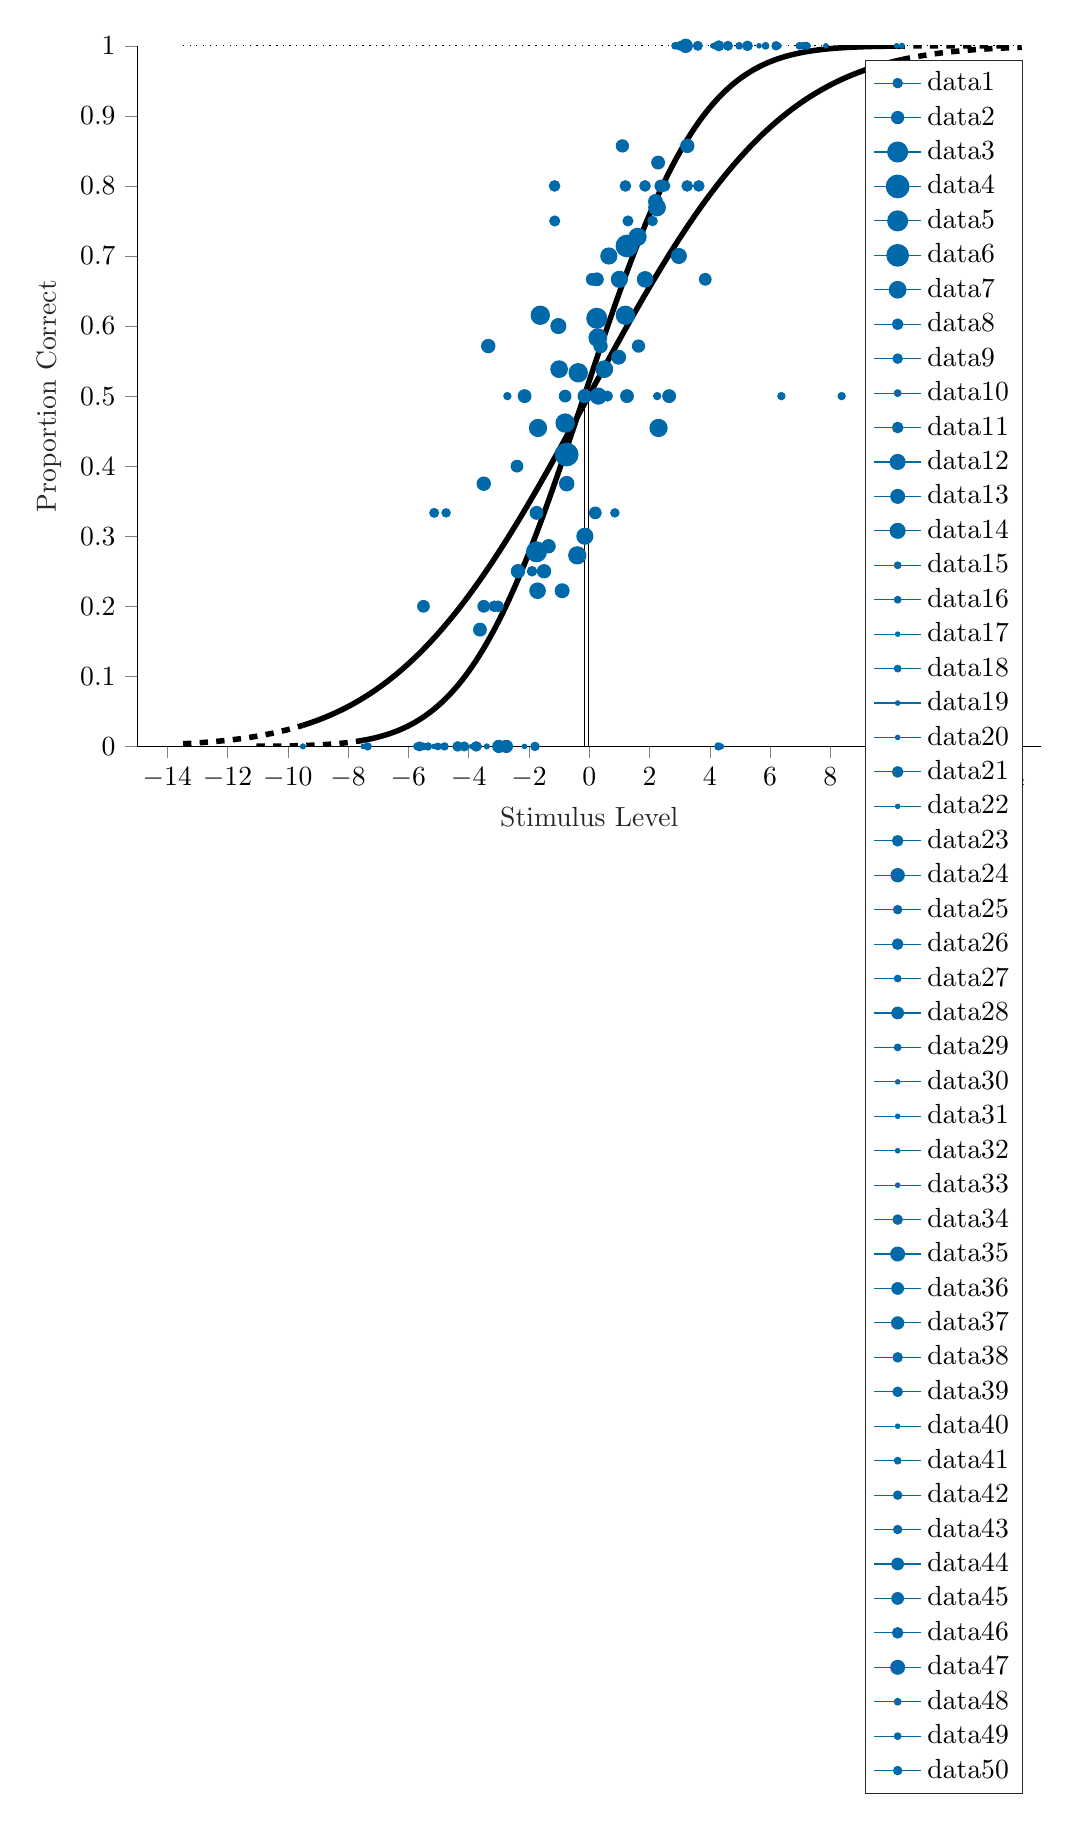
\begin{tikzpicture}

\begin{axis}[%
width=4.521in,
height=3.503in,
at={(0.758in,0.544in)},
scale only axis,
xmin=-15,
xmax=15,
tick align=outside,
xlabel style={font=\color{white!15!black}},
xlabel={Stimulus Level},
ymin=0,
ymax=1,
ylabel style={font=\color{white!15!black}},
ylabel={Proportion Correct},
axis background/.style={fill=white},
axis x line*=bottom,
axis y line*=left,
legend style={legend cell align=left, align=left, draw=white!15!black}
]
\addplot [color=mycolor1, draw=none, mark size=1.7pt, mark=*, mark options={solid, mycolor1}]
  table[row sep=crcr]{%
-3.75	0\\
};
\addlegendentry{data1}

\addplot [color=mycolor1, draw=none, mark size=2.2pt, mark=*, mark options={solid, mycolor1}]
  table[row sep=crcr]{%
-2.75	0\\
};
\addlegendentry{data2}

\addplot [color=mycolor1, draw=none, mark size=3.6pt, mark=*, mark options={solid, mycolor1}]
  table[row sep=crcr]{%
-1.75	0.277777777777778\\
};
\addlegendentry{data3}

\addplot [color=mycolor1, draw=none, mark size=4.1pt, mark=*, mark options={solid, mycolor1}]
  table[row sep=crcr]{%
-0.75	0.416666666666667\\
};
\addlegendentry{data4}

\addplot [color=mycolor1, draw=none, mark size=3.6pt, mark=*, mark options={solid, mycolor1}]
  table[row sep=crcr]{%
0.25	0.611111111111111\\
};
\addlegendentry{data5}

\addplot [color=mycolor1, draw=none, mark size=3.9pt, mark=*, mark options={solid, mycolor1}]
  table[row sep=crcr]{%
1.25	0.714285714285714\\
};
\addlegendentry{data6}

\addplot [color=mycolor1, draw=none, mark size=3.0pt, mark=*, mark options={solid, mycolor1}]
  table[row sep=crcr]{%
2.25	0.769230769230769\\
};
\addlegendentry{data7}

\addplot [color=mycolor1, draw=none, mark size=1.9pt, mark=*, mark options={solid, mycolor1}]
  table[row sep=crcr]{%
3.25	0.8\\
};
\addlegendentry{data8}

\addplot [color=mycolor1, draw=none, mark size=1.7pt, mark=*, mark options={solid, mycolor1}]
  table[row sep=crcr]{%
5.25	1\\
};
\addlegendentry{data9}

\addplot [color=mycolor1, draw=none, mark size=1.2pt, mark=*, mark options={solid, mycolor1}]
  table[row sep=crcr]{%
-5.025	0\\
};
\addlegendentry{data10}

\addplot [color=mycolor1, draw=none, mark size=1.9pt, mark=*, mark options={solid, mycolor1}]
  table[row sep=crcr]{%
-3.025	0.2\\
};
\addlegendentry{data11}

\addplot [color=mycolor1, draw=none, mark size=2.7pt, mark=*, mark options={solid, mycolor1}]
  table[row sep=crcr]{%
-1.025	0.6\\
};
\addlegendentry{data12}

\addplot [color=mycolor1, draw=none, mark size=2.5pt, mark=*, mark options={solid, mycolor1}]
  table[row sep=crcr]{%
0.975	0.555555555555556\\
};
\addlegendentry{data13}

\addplot [color=mycolor1, draw=none, mark size=2.7pt, mark=*, mark options={solid, mycolor1}]
  table[row sep=crcr]{%
2.975	0.7\\
};
\addlegendentry{data14}

\addplot [color=mycolor1, draw=none, mark size=1.2pt, mark=*, mark options={solid, mycolor1}]
  table[row sep=crcr]{%
4.975	1\\
};
\addlegendentry{data15}

\addplot [color=mycolor1, draw=none, mark size=1.2pt, mark=*, mark options={solid, mycolor1}]
  table[row sep=crcr]{%
6.975	1\\
};
\addlegendentry{data16}

\addplot [color=mycolor1, draw=none, mark size=0.8pt, mark=*, mark options={solid, mycolor1}]
  table[row sep=crcr]{%
-5.75	0\\
};
\addlegendentry{data17}

\addplot [color=mycolor1, draw=none, mark size=1.2pt, mark=*, mark options={solid, mycolor1}]
  table[row sep=crcr]{%
4.25	1\\
};
\addlegendentry{data18}

\addplot [color=mycolor1, draw=none, mark size=0.8pt, mark=*, mark options={solid, mycolor1}]
  table[row sep=crcr]{%
-5.15	0\\
};
\addlegendentry{data19}

\addplot [color=mycolor1, draw=none, mark size=0.8pt, mark=*, mark options={solid, mycolor1}]
  table[row sep=crcr]{%
-4.15	0\\
};
\addlegendentry{data20}

\addplot [color=mycolor1, draw=none, mark size=1.9pt, mark=*, mark options={solid, mycolor1}]
  table[row sep=crcr]{%
-3.15	0.2\\
};
\addlegendentry{data21}

\addplot [color=mycolor1, draw=none, mark size=0.8pt, mark=*, mark options={solid, mycolor1}]
  table[row sep=crcr]{%
-2.15	0\\
};
\addlegendentry{data22}

\addplot [color=mycolor1, draw=none, mark size=1.9pt, mark=*, mark options={solid, mycolor1}]
  table[row sep=crcr]{%
-1.15	0.8\\
};
\addlegendentry{data23}

\addplot [color=mycolor1, draw=none, mark size=2.4pt, mark=*, mark options={solid, mycolor1}]
  table[row sep=crcr]{%
-0.15	0.5\\
};
\addlegendentry{data24}

\addplot [color=mycolor1, draw=none, mark size=1.5pt, mark=*, mark options={solid, mycolor1}]
  table[row sep=crcr]{%
0.85	0.333333333333333\\
};
\addlegendentry{data25}

\addplot [color=mycolor1, draw=none, mark size=1.9pt, mark=*, mark options={solid, mycolor1}]
  table[row sep=crcr]{%
1.85	0.8\\
};
\addlegendentry{data26}

\addplot [color=mycolor1, draw=none, mark size=1.2pt, mark=*, mark options={solid, mycolor1}]
  table[row sep=crcr]{%
2.85	1\\
};
\addlegendentry{data27}

\addplot [color=mycolor1, draw=none, mark size=2.1pt, mark=*, mark options={solid, mycolor1}]
  table[row sep=crcr]{%
3.85	0.666666666666667\\
};
\addlegendentry{data28}

\addplot [color=mycolor1, draw=none, mark size=1.2pt, mark=*, mark options={solid, mycolor1}]
  table[row sep=crcr]{%
5.85	1\\
};
\addlegendentry{data29}

\addplot [color=mycolor1, draw=none, mark size=0.8pt, mark=*, mark options={solid, mycolor1}]
  table[row sep=crcr]{%
7.85	1\\
};
\addlegendentry{data30}

\addplot [color=mycolor1, draw=none, mark size=0.8pt, mark=*, mark options={solid, mycolor1}]
  table[row sep=crcr]{%
-4.9	0\\
};
\addlegendentry{data31}

\addplot [color=mycolor1, draw=none, mark size=0.8pt, mark=*, mark options={solid, mycolor1}]
  table[row sep=crcr]{%
-3.9	0\\
};
\addlegendentry{data32}

\addplot [color=mycolor1, draw=none, mark size=0.8pt, mark=*, mark options={solid, mycolor1}]
  table[row sep=crcr]{%
-2.9	0\\
};
\addlegendentry{data33}

\addplot [color=mycolor1, draw=none, mark size=1.7pt, mark=*, mark options={solid, mycolor1}]
  table[row sep=crcr]{%
-1.9	0.25\\
};
\addlegendentry{data34}

\addplot [color=mycolor1, draw=none, mark size=2.5pt, mark=*, mark options={solid, mycolor1}]
  table[row sep=crcr]{%
-0.9	0.222222222222222\\
};
\addlegendentry{data35}

\addplot [color=mycolor1, draw=none, mark size=2.1pt, mark=*, mark options={solid, mycolor1}]
  table[row sep=crcr]{%
0.0999999999999996	0.666666666666667\\
};
\addlegendentry{data36}

\addplot [color=mycolor1, draw=none, mark size=2.2pt, mark=*, mark options={solid, mycolor1}]
  table[row sep=crcr]{%
1.1	0.857142857142857\\
};
\addlegendentry{data37}

\addplot [color=mycolor1, draw=none, mark size=1.7pt, mark=*, mark options={solid, mycolor1}]
  table[row sep=crcr]{%
2.1	0.75\\
};
\addlegendentry{data38}

\addplot [color=mycolor1, draw=none, mark size=1.7pt, mark=*, mark options={solid, mycolor1}]
  table[row sep=crcr]{%
3.1	1\\
};
\addlegendentry{data39}

\addplot [color=mycolor1, draw=none, mark size=0.8pt, mark=*, mark options={solid, mycolor1}]
  table[row sep=crcr]{%
4.1	1\\
};
\addlegendentry{data40}

\addplot [color=mycolor1, draw=none, mark size=1.2pt, mark=*, mark options={solid, mycolor1}]
  table[row sep=crcr]{%
7.1	1\\
};
\addlegendentry{data41}

\addplot [color=mycolor1, draw=none, mark size=1.5pt, mark=*, mark options={solid, mycolor1}]
  table[row sep=crcr]{%
-2.8	0\\
};
\addlegendentry{data42}

\addplot [color=mycolor1, draw=none, mark size=1.5pt, mark=*, mark options={solid, mycolor1}]
  table[row sep=crcr]{%
-1.8	0\\
};
\addlegendentry{data43}

\addplot [color=mycolor1, draw=none, mark size=2.1pt, mark=*, mark options={solid, mycolor1}]
  table[row sep=crcr]{%
-0.8	0.5\\
};
\addlegendentry{data44}

\addplot [color=mycolor1, draw=none, mark size=2.1pt, mark=*, mark options={solid, mycolor1}]
  table[row sep=crcr]{%
0.2	0.333333333333333\\
};
\addlegendentry{data45}

\addplot [color=mycolor1, draw=none, mark size=1.9pt, mark=*, mark options={solid, mycolor1}]
  table[row sep=crcr]{%
1.2	0.8\\
};
\addlegendentry{data46}

\addplot [color=mycolor1, draw=none, mark size=2.5pt, mark=*, mark options={solid, mycolor1}]
  table[row sep=crcr]{%
2.2	0.777777777777778\\
};
\addlegendentry{data47}

\addplot [color=mycolor1, draw=none, mark size=1.2pt, mark=*, mark options={solid, mycolor1}]
  table[row sep=crcr]{%
3.2	1\\
};
\addlegendentry{data48}

\addplot [color=mycolor1, draw=none, mark size=1.2pt, mark=*, mark options={solid, mycolor1}]
  table[row sep=crcr]{%
4.2	1\\
};
\addlegendentry{data49}

\addplot [color=mycolor1, draw=none, mark size=1.5pt, mark=*, mark options={solid, mycolor1}]
  table[row sep=crcr]{%
6.2	1\\
};
\addlegendentry{data50}

\addplot [color=mycolor1, draw=none, mark size=0.8pt, mark=*, mark options={solid, mycolor1}, forget plot]
  table[row sep=crcr]{%
10.2	1\\
};
\addplot [color=mycolor1, draw=none, mark size=0.8pt, mark=*, mark options={solid, mycolor1}, forget plot]
  table[row sep=crcr]{%
-7.5	0\\
};
\addplot [color=mycolor1, draw=none, mark size=1.2pt, mark=*, mark options={solid, mycolor1}, forget plot]
  table[row sep=crcr]{%
-5.5	0\\
};
\addplot [color=mycolor1, draw=none, mark size=2.4pt, mark=*, mark options={solid, mycolor1}, forget plot]
  table[row sep=crcr]{%
-3.5	0.375\\
};
\addplot [color=mycolor1, draw=none, mark size=2.4pt, mark=*, mark options={solid, mycolor1}, forget plot]
  table[row sep=crcr]{%
-1.5	0.25\\
};
\addplot [color=mycolor1, draw=none, mark size=3.0pt, mark=*, mark options={solid, mycolor1}, forget plot]
  table[row sep=crcr]{%
0.5	0.538461538461538\\
};
\addplot [color=mycolor1, draw=none, mark size=1.9pt, mark=*, mark options={solid, mycolor1}, forget plot]
  table[row sep=crcr]{%
2.5	0.8\\
};
\addplot [color=mycolor1, draw=none, mark size=1.7pt, mark=*, mark options={solid, mycolor1}, forget plot]
  table[row sep=crcr]{%
-4.365	0\\
};
\addplot [color=mycolor1, draw=none, mark size=2.4pt, mark=*, mark options={solid, mycolor1}, forget plot]
  table[row sep=crcr]{%
-2.365	0.25\\
};
\addplot [color=mycolor1, draw=none, mark size=3.3pt, mark=*, mark options={solid, mycolor1}, forget plot]
  table[row sep=crcr]{%
-0.365	0.533333333333333\\
};
\addplot [color=mycolor1, draw=none, mark size=2.2pt, mark=*, mark options={solid, mycolor1}, forget plot]
  table[row sep=crcr]{%
1.635	0.571428571428571\\
};
\addplot [color=mycolor1, draw=none, mark size=1.9pt, mark=*, mark options={solid, mycolor1}, forget plot]
  table[row sep=crcr]{%
3.635	0.8\\
};
\addplot [color=mycolor1, draw=none, mark size=0.8pt, mark=*, mark options={solid, mycolor1}, forget plot]
  table[row sep=crcr]{%
5.635	1\\
};
\addplot [color=mycolor1, draw=none, mark size=2.2pt, mark=*, mark options={solid, mycolor1}, forget plot]
  table[row sep=crcr]{%
-3	0\\
};
\addplot [color=mycolor1, draw=none, mark size=3.0pt, mark=*, mark options={solid, mycolor1}, forget plot]
  table[row sep=crcr]{%
-1	0.538461538461538\\
};
\addplot [color=mycolor1, draw=none, mark size=2.9pt, mark=*, mark options={solid, mycolor1}, forget plot]
  table[row sep=crcr]{%
1	0.666666666666667\\
};
\addplot [color=mycolor1, draw=none, mark size=1.5pt, mark=*, mark options={solid, mycolor1}, forget plot]
  table[row sep=crcr]{%
3	1\\
};
\addplot [color=mycolor1, draw=none, mark size=1.5pt, mark=*, mark options={solid, mycolor1}, forget plot]
  table[row sep=crcr]{%
-4.75	0.333333333333333\\
};
\addplot [color=black, line width=2.0pt, forget plot]
  table[row sep=crcr]{%
-7.5	0.0087420877707031\\
-7.48228228228228	0.00887910975213292\\
-7.46456456456456	0.00901801010169164\\
-7.44684684684685	0.00915880992443155\\
-7.42912912912913	0.00930153048784899\\
-7.41141141141141	0.00944619322198411\\
-7.39369369369369	0.00959281971950041\\
-7.37597597597598	0.00974143173574372\\
-7.35825825825826	0.00989205118878049\\
-7.34054054054054	0.0100447001594149\\
-7.32282282282282	0.0101994008911844\\
-7.30510510510511	0.0103561757903341\\
-7.28738738738739	0.0105150474257686\\
-7.26966966966967	0.0106760385289818\\
-7.25195195195195	0.0108391719939646\\
-7.23423423423423	0.0110044708770888\\
-7.21651651651652	0.0111719583969691\\
-7.1987987987988	0.0113416579343006\\
-7.18108108108108	0.0115135930316734\\
-7.16336336336336	0.0116877873933628\\
-7.14564564564565	0.0118642648850959\\
-7.12792792792793	0.0120430495337924\\
-7.11021021021021	0.0122241655272822\\
-7.09249249249249	0.0124076372139969\\
-7.07477477477477	0.0125934891026359\\
-7.05705705705706	0.0127817458618076\\
-7.03933933933934	0.0129724323196442\\
-7.02162162162162	0.0131655734633905\\
-7.0039039039039	0.0133611944389657\\
-6.98618618618619	0.0135593205504996\\
-6.96846846846847	0.013759977259841\\
-6.95075075075075	0.0139631901860389\\
-6.93303303303303	0.0141689851047966\\
-6.91531531531531	0.0143773879478978\\
-6.8975975975976	0.0145884248026044\\
-6.87987987987988	0.014802121911027\\
-6.86216216216216	0.0150185056694653\\
-6.84444444444444	0.0152376026277215\\
-6.82672672672673	0.0154594394883833\\
-6.80900900900901	0.0156840431060783\\
-6.79129129129129	0.0159114404866987\\
-6.77357357357357	0.0161416587865962\\
-6.75585585585586	0.0163747253117472\\
-6.73813813813814	0.0166106675168874\\
-6.72042042042042	0.0168495130046162\\
-6.7027027027027	0.0170912895244702\\
-6.68498498498499	0.017336024971966\\
-6.66726726726727	0.0175837473876119\\
-6.64954954954955	0.0178344849558881\\
-6.63183183183183	0.0180882660041954\\
-6.61411411411411	0.0183451190017718\\
-6.5963963963964	0.0186050725585782\\
-6.57867867867868	0.0188681554241505\\
-6.56096096096096	0.0191343964864203\\
-6.54324324324324	0.0194038247705027\\
-6.52552552552553	0.0196764694374513\\
-6.50780780780781	0.0199523597829805\\
-6.49009009009009	0.0202315252361544\\
-6.47237237237237	0.0205139953580423\\
-6.45465465465465	0.0207997998403415\\
-6.43693693693694	0.0210889685039651\\
-6.41921921921922	0.0213815312975973\\
-6.4015015015015	0.0216775182962139\\
-6.38378378378378	0.0219769596995695\\
-6.36606606606607	0.0222798858306491\\
-6.34834834834835	0.0225863271340866\\
-6.33063063063063	0.0228963141745481\\
-6.31291291291291	0.0232098776350806\\
-6.29519519519519	0.0235270483154263\\
-6.27747747747748	0.0238478571303007\\
-6.25975975975976	0.0241723351076375\\
-6.24204204204204	0.0245005133867967\\
-6.22432432432432	0.0248324232167386\\
-6.20660660660661	0.0251680959541614\\
-6.18888888888889	0.0255075630616042\\
-6.17117117117117	0.0258508561055141\\
-6.15345345345345	0.0261980067542773\\
-6.13573573573574	0.0265490467762153\\
-6.11801801801802	0.0269040080375446\\
-6.1003003003003	0.0272629225003011\\
-6.08258258258258	0.0276258222202279\\
-6.06486486486487	0.0279927393446277\\
-6.04714714714715	0.0283637061101795\\
-6.02942942942943	0.0287387548407182\\
-6.01171171171171	0.0291179179449793\\
-5.99399399399399	0.0295012279143066\\
-5.97627627627628	0.0298887173203246\\
-5.95855855855856	0.030280418812574\\
-5.94084084084084	0.0306763651161117\\
-5.92312312312312	0.0310765890290743\\
-5.90540540540541	0.031481123420206\\
-5.88768768768769	0.0318900012263496\\
-5.86996996996997	0.0323032554499022\\
-5.85225225225225	0.0327209191562348\\
-5.83453453453453	0.0331430254710755\\
-5.81681681681682	0.0335696075778568\\
-5.7990990990991	0.0340006987150278\\
-5.78138138138138	0.0344363321733299\\
-5.76366366366366	0.0348765412930364\\
-5.74594594594595	0.0353213594611577\\
-5.72822822822823	0.0357708201086099\\
-5.71051051051051	0.0362249567073479\\
-5.69279279279279	0.0366838027674641\\
-5.67507507507507	0.037147391834251\\
-5.65735735735736	0.0376157574852286\\
-5.63963963963964	0.0380889333271376\\
-5.62192192192192	0.0385669529928969\\
-5.6042042042042	0.039049850138527\\
-5.58648648648649	0.0395376584400382\\
-5.56876876876877	0.0400304115902852\\
-5.55105105105105	0.0405281432957869\\
-5.53333333333333	0.0410308872735122\\
-5.51561561561562	0.0415386772476321\\
-5.4978978978979	0.0420515469462381\\
-5.48018018018018	0.0425695300980272\\
-5.46246246246246	0.0430926604289534\\
-5.44474474474475	0.0436209716588466\\
-5.42702702702703	0.0441544974979982\\
-5.40930930930931	0.0446932716437147\\
-5.39159159159159	0.0452373277768386\\
-5.37387387387387	0.0457866995582373\\
-5.35615615615616	0.0463414206252605\\
-5.33843843843844	0.0469015245881658\\
-5.32072072072072	0.0474670450265134\\
-5.303003003003	0.0480380154855292\\
-5.28528528528529	0.0486144694724385\\
-5.26756756756757	0.0491964404527682\\
-5.24984984984985	0.0497839618466195\\
-5.23213213213213	0.0503770670249112\\
-5.21441441441442	0.0509757893055933\\
-5.1966966966967	0.0515801619498317\\
-5.17897897897898	0.0521902181581645\\
-5.16126126126126	0.0528059910666301\\
-5.14354354354354	0.0534275137428666\\
-5.12582582582583	0.0540548191821855\\
-5.10810810810811	0.054687940303616\\
-5.09039039039039	0.0553269099459247\\
-5.07267267267267	0.0559717608636081\\
-5.05495495495495	0.0566225257228585\\
-5.03723723723724	0.0572792370975064\\
-5.01951951951952	0.057941927464936\\
-5.0018018018018	0.0586106292019776\\
-4.98408408408408	0.0592853745807746\\
-4.96636636636637	0.0599661957646283\\
-4.94864864864865	0.0606531248038184\\
-4.93093093093093	0.0613461936314015\\
-4.91321321321321	0.0620454340589873\\
-4.8954954954955	0.0627508777724928\\
-4.87777777777778	0.0634625563278762\\
-4.86006006006006	0.064180501146849\\
-4.84234234234234	0.0649047435125693\\
-4.82462462462462	0.0656353145653139\\
-4.80690690690691	0.0663722452981336\\
-4.78918918918919	0.0671155665524876\\
-4.77147147147147	0.0678653090138619\\
-4.75375375375375	0.0686215032073694\\
-4.73603603603604	0.0693841794933336\\
-4.71831831831832	0.0701533680628555\\
-4.7006006006006	0.0709290989333665\\
-4.68288288288288	0.071711401944164\\
-4.66516516516517	0.072500306751935\\
-4.64744744744745	0.0732958428262641\\
-4.62972972972973	0.0740980394451298\\
-4.61201201201201	0.0749069256903872\\
-4.59429429429429	0.0757225304432397\\
-4.57657657657658	0.0765448823796989\\
-4.55885885885886	0.0773740099660344\\
-4.54114114114114	0.0782099414542138\\
-4.52342342342342	0.079052704877333\\
-4.50570570570571	0.0799023280450385\\
-4.48798798798799	0.0807588385389417\\
-4.47027027027027	0.0816222637080262\\
-4.45255255255255	0.0824926306640485\\
-4.43483483483483	0.0833699662769328\\
-4.41711711711712	0.0842542971701618\\
-4.3993993993994	0.0851456497161617\\
-4.38168168168168	0.0860440500316855\\
-4.36396396396396	0.0869495239731914\\
-4.34624624624625	0.087862097132221\\
-4.32852852852853	0.0887817948307754\\
-4.31081081081081	0.0897086421166907\\
-4.29309309309309	0.0906426637590134\\
-4.27537537537538	0.0915838842433778\\
-4.25765765765766	0.0925323277673846\\
-4.23993993993994	0.0934880182359813\\
-4.22222222222222	0.0944509792568474\\
-4.2045045045045	0.0954212341357821\\
-4.18678678678679	0.0963988058720985\\
-4.16906906906907	0.0973837171540221\\
-4.15135135135135	0.0983759903540967\\
-4.13363363363363	0.0993756475245973\\
-4.11591591591592	0.100382710392951\\
-4.0981981981982	0.101397200357167\\
-4.08048048048048	0.102419138481277\\
-4.06276276276276	0.103448545490785\\
-4.04504504504505	0.104485441768128\\
-4.02732732732733	0.105529847348153\\
-4.00960960960961	0.1065817819136\\
-3.99189189189189	0.107641264790608\\
-3.97417417417417	0.108708314944227\\
-3.95645645645646	0.10978295097395\\
-3.93873873873874	0.110865191109264\\
-3.92102102102102	0.111955053205212\\
-3.9033033033033	0.113052554737978\\
-3.88558558558559	0.114157712800488\\
-3.86786786786787	0.115270544098038\\
-3.85015015015015	0.116391064943928\\
-3.83243243243243	0.117519291255137\\
-3.81471471471471	0.118655238548003\\
-3.796996996997	0.119798921933937\\
-3.77927927927928	0.120950356115158\\
-3.76156156156156	0.122109555380455\\
-3.74384384384384	0.123276533600969\\
-3.72612612612613	0.124451304226008\\
-3.70840840840841	0.125633880278891\\
-3.69069069069069	0.126824274352814\\
-3.67297297297297	0.128022498606749\\
-3.65525525525526	0.129228564761374\\
-3.63753753753754	0.130442484095037\\
-3.61981981981982	0.131664267439742\\
-3.6021021021021	0.132893925177181\\
-3.58438438438438	0.13413146723479\\
-3.56666666666667	0.135376903081845\\
-3.54894894894895	0.136630241725592\\
-3.53123123123123	0.13789149170741\\
-3.51351351351351	0.13916066109902\\
-3.4957957957958	0.140437757498725\\
-3.47807807807808	0.141722788027689\\
-3.46036036036036	0.143015759326259\\
-3.44264264264264	0.144316677550329\\
-3.42492492492492	0.14562554836774\\
-3.40720720720721	0.146942376954729\\
-3.38948948948949	0.148267167992414\\
-3.37177177177177	0.149599925663331\\
-3.35405405405405	0.150940653648013\\
-3.33633633633634	0.152289355121611\\
-3.31861861861862	0.153646032750566\\
-3.3009009009009	0.155010688689328\\
-3.28318318318318	0.156383324577124\\
-3.26546546546547	0.157763941534771\\
-3.24774774774775	0.159152540161545\\
-3.23003003003003	0.160549120532096\\
-3.21231231231231	0.161953682193415\\
-3.1945945945946	0.16336622416186\\
-3.17687687687688	0.164786744920222\\
-3.15915915915916	0.166215242414861\\
-3.14144144144144	0.167651714052882\\
-3.12372372372372	0.169096156699379\\
-3.10600600600601	0.170548566674723\\
-3.08828828828829	0.172008939751921\\
-3.07057057057057	0.173477271154017\\
-3.05285285285285	0.174953555551569\\
-3.03513513513514	0.176437787060167\\
-3.01741741741742	0.177929959238028\\
-2.9996996996997	0.179430065083641\\
-2.98198198198198	0.180938097033473\\
-2.96426426426426	0.182454046959746\\
-2.94654654654655	0.183977906168269\\
-2.92882882882883	0.185509665396337\\
-2.91111111111111	0.187049314810692\\
-2.89339339339339	0.188596844005551\\
-2.87567567567568	0.190152242000697\\
-2.85795795795796	0.191715497239643\\
-2.84024024024024	0.193286597587851\\
-2.82252252252252	0.194865530331032\\
-2.8048048048048	0.196452282173502\\
-2.78708708708709	0.198046839236617\\
-2.76936936936937	0.199649187057267\\
-2.75165165165165	0.201259310586451\\
-2.73393393393393	0.202877194187915\\
-2.71621621621622	0.20450282163686\\
-2.6984984984985	0.206136176118731\\
-2.68078078078078	0.207777240228066\\
-2.66306306306306	0.209425995967425\\
-2.64534534534535	0.211082424746395\\
-2.62762762762763	0.212746507380659\\
-2.60990990990991	0.214418224091146\\
-2.59219219219219	0.216097554503257\\
-2.57447447447448	0.217784477646163\\
-2.55675675675676	0.219478971952176\\
-2.53903903903904	0.221181015256205\\
-2.52132132132132	0.222890584795278\\
-2.5036036036036	0.224607657208148\\
-2.48588588588589	0.226332208534974\\
-2.46816816816817	0.228064214217083\\
-2.45045045045045	0.2298036490968\\
-2.43273273273273	0.231550487417371\\
-2.41501501501502	0.233304702822956\\
-2.3972972972973	0.235066268358698\\
-2.37957957957958	0.236835156470882\\
-2.36186186186186	0.238611339007165\\
-2.34414414414414	0.240394787216889\\
-2.32642642642643	0.242185471751479\\
-2.30870870870871	0.243983362664909\\
-2.29099099099099	0.245788429414266\\
-2.27327327327327	0.24760064086038\\
-2.25555555555556	0.249419965268545\\
-2.23783783783784	0.251246370309316\\
-2.22012012012012	0.253079823059392\\
-2.2024024024024	0.254920290002579\\
-2.18468468468468	0.256767737030833\\
-2.16696696696697	0.258622129445388\\
-2.14924924924925	0.260483431957968\\
-2.13153153153153	0.262351608692076\\
-2.11381381381381	0.26422662318437\\
-2.0960960960961	0.26610843838612\\
-2.07837837837838	0.267997016664751\\
-2.06066066066066	0.269892319805458\\
-2.04294294294294	0.271794309012923\\
-2.02522522522522	0.273702944913092\\
-2.00750750750751	0.275618187555054\\
-1.98978978978979	0.277539996412992\\
-1.97207207207207	0.279468330388221\\
-1.95435435435436	0.281403147811304\\
-1.93663663663664	0.283344406444261\\
-1.91891891891892	0.285292063482845\\
-1.9012012012012	0.287246075558915\\
-1.88348348348348	0.289206398742886\\
-1.86576576576577	0.291172988546255\\
-1.84804804804805	0.293145799924221\\
-1.83033033033033	0.295124787278375\\
-1.81261261261261	0.297109904459481\\
-1.7948948948949	0.299101104770333\\
-1.77717717717718	0.301098340968697\\
-1.75945945945946	0.303101565270328\\
-1.74174174174174	0.305110729352075\\
-1.72402402402402	0.307125784355063\\
-1.70630630630631	0.309146680887954\\
-1.68858858858859	0.311173369030291\\
-1.67087087087087	0.313205798335919\\
-1.65315315315315	0.315243917836485\\
-1.63543543543544	0.317287676045024\\
-1.61771771771772	0.319337020959608\\
-1.6	0.321391900067093\\
-1.58228228228228	0.323452260346927\\
-1.56456456456456	0.325518048275045\\
-1.54684684684685	0.327589209827836\\
-1.52912912912913	0.32966569048619\\
-1.51141141141141	0.331747435239619\\
-1.49369369369369	0.333834388590455\\
-1.47597597597598	0.335926494558116\\
-1.45825825825826	0.338023696683463\\
-1.44054054054054	0.340125938033209\\
-1.42282282282282	0.342233161204421\\
-1.4051051051051	0.344345308329083\\
-1.38738738738739	0.346462321078732\\
-1.36966966966967	0.348584140669177\\
-1.35195195195195	0.350710707865271\\
-1.33423423423424	0.352841962985768\\
-1.31651651651652	0.354977845908246\\
-1.2987987987988	0.357118296074093\\
-1.28108108108108	0.359263252493569\\
-1.26336336336336	0.361412653750936\\
-1.24564564564565	0.363566438009646\\
-1.22792792792793	0.365724543017606\\
-1.21021021021021	0.367886906112503\\
-1.19249249249249	0.370053464227192\\
-1.17477477477478	0.372224153895159\\
-1.15705705705706	0.374398911256028\\
-1.13933933933934	0.376577672061152\\
-1.12162162162162	0.37876037167925\\
-1.1039039039039	0.380946945102113\\
-1.08618618618619	0.383137326950365\\
-1.06846846846847	0.385331451479291\\
-1.05075075075075	0.387529252584711\\
-1.03303303303303	0.389730663808926\\
-1.01531531531532	0.391935618346708\\
-0.997597597597598	0.394144049051356\\
-0.97987987987988	0.396355888440797\\
-0.962162162162162	0.398571068703749\\
-0.944444444444445	0.400789521705934\\
-0.926726726726727	0.403011178996343\\
-0.90900900900901	0.405235971813548\\
-0.891291291291292	0.407463831092074\\
-0.873573573573573	0.409694687468812\\
-0.855855855855856	0.411928471289479\\
-0.838138138138138	0.414165112615135\\
-0.820420420420421	0.416404541228735\\
-0.802702702702703	0.41864668664173\\
-0.784984984984985	0.420891478100717\\
-0.767267267267267	0.423138844594125\\
-0.74954954954955	0.425388714858947\\
-0.731831831831832	0.427641017387509\\
-0.714114114114115	0.429895680434288\\
-0.696396396396397	0.432152632022754\\
-0.678678678678678	0.434411799952265\\
-0.660960960960961	0.436673111804988\\
-0.643243243243243	0.438936494952858\\
-0.625525525525526	0.441201876564578\\
-0.607807807807808	0.44346918361264\\
-0.59009009009009	0.445738342880391\\
-0.572372372372373	0.448009280969117\\
-0.554654654654655	0.450281924305169\\
-0.536936936936938	0.452556199147112\\
-0.51921921921922	0.454832031592897\\
-0.501501501501502	0.457109347587069\\
-0.483783783783784	0.459388072927994\\
-0.466066066066066	0.461668133275111\\
-0.448348348348349	0.463949454156204\\
-0.430630630630631	0.466231960974707\\
-0.412912912912913	0.468515579017012\\
-0.395195195195195	0.47080023345981\\
-0.377477477477478	0.473085849377447\\
-0.35975975975976	0.475372351749291\\
-0.342042042042043	0.477659665467122\\
-0.324324324324325	0.479947715342535\\
-0.306606606606607	0.482236426114348\\
-0.28888888888889	0.484525722456036\\
-0.271171171171171	0.486815528983165\\
-0.253453453453454	0.489105770260838\\
-0.235735735735735	0.491396370811154\\
-0.218018018018018	0.493687255120665\\
-0.200300300300301	0.495978347647849\\
-0.182582582582583	0.49826957283058\\
-0.164864864864866	0.500560855093605\\
-0.147147147147147	0.502852118856022\\
-0.12942942942943	0.505143288538762\\
-0.111711711711712	0.507434288572064\\
-0.0939939939939949	0.509725043402953\\
-0.0762762762762774	0.51201547750272\\
-0.0585585585585582	0.514305515374384\\
-0.0408408408408407	0.516595081560166\\
-0.0231231231231233	0.518884100648942\\
-0.00540540540540579	0.521172497283698\\
0.0123123123123117	0.523460196168968\\
0.03003003003003	0.525747122078274\\
0.0477477477477475	0.528033199861538\\
0.0654654654654649	0.530318354452496\\
0.0831831831831824	0.532602510876091\\
0.1009009009009	0.534885594255851\\
0.118618618618618	0.537167529821256\\
0.136336336336337	0.53944824291508\\
0.154054054054054	0.54172765900072\\
0.171771771771771	0.544005703669502\\
0.189489489489489	0.546282302647969\\
0.207207207207207	0.548557381805146\\
0.224924924924925	0.550830867159777\\
0.242642642642642	0.553102684887544\\
0.26036036036036	0.555372761328256\\
0.278078078078077	0.557641022993014\\
0.295795795795796	0.559907396571345\\
0.313513513513513	0.562171808938308\\
0.33123123123123	0.564434187161572\\
0.348948948948949	0.566694458508455\\
0.366666666666666	0.568952550452943\\
0.384384384384385	0.571208390682661\\
0.402102102102102	0.573461907105819\\
0.41981981981982	0.575713027858119\\
0.437537537537537	0.577961681309625\\
0.455255255255254	0.580207796071592\\
0.472972972972973	0.582451301003262\\
0.49069069069069	0.584692125218611\\
0.508408408408409	0.586930198093065\\
0.526126126126126	0.589165449270163\\
0.543843843843844	0.591397808668185\\
0.561561561561561	0.593627206486731\\
0.579279279279278	0.595853573213252\\
0.596996996996996	0.598076839629542\\
0.614714714714713	0.600296936818176\\
0.632432432432431	0.6025137961689\\
0.65015015015015	0.604727349384978\\
0.667867867867868	0.606937528489474\\
0.685585585585585	0.609144265831501\\
0.703303303303304	0.611347494092401\\
0.72102102102102	0.613547146291883\\
0.738738738738739	0.615743155794102\\
0.756456456456455	0.61793545631368\\
0.774174174174174	0.620123981921676\\
0.791891891891892	0.622308667051497\\
0.809609609609609	0.62448944650475\\
0.827327327327327	0.626666255457036\\
0.845045045045044	0.628839029463685\\
0.862762762762763	0.63100770446543\\
0.880480480480481	0.633172216794018\\
0.898198198198198	0.635332503177762\\
0.915915915915916	0.637488500747026\\
0.933633633633633	0.639640147039654\\
0.951351351351351	0.641787380006323\\
0.96906906906907	0.643930138015842\\
0.986786786786785	0.646068359860375\\
1.0045045045045	0.648201984760609\\
1.02222222222222	0.650330952370841\\
1.03993993993994	0.652455202784011\\
1.05765765765766	0.654574676536652\\
1.07537537537537	0.656689314613781\\
1.09309309309309	0.65879905845372\\
1.11081081081081	0.660903849952834\\
1.12852852852853	0.663003631470217\\
1.14624624624625	0.665098345832286\\
1.16396396396396	0.66718793633732\\
1.18168168168168	0.669272346759909\\
1.1993993993994	0.671351521355349\\
1.21711711711712	0.673425404863942\\
1.23483483483484	0.675493942515237\\
1.25255255255255	0.677557080032187\\
1.27027027027027	0.679614763635237\\
1.28798798798799	0.681666940046326\\
1.30570570570571	0.683713556492826\\
1.32342342342342	0.685754560711389\\
1.34114114114114	0.687789900951727\\
1.35885885885886	0.689819525980311\\
1.37657657657657	0.691843385083991\\
1.39429429429429	0.693861428073538\\
1.41201201201201	0.695873605287104\\
1.42972972972973	0.697879867593608\\
1.44744744744745	0.699880166396038\\
1.46516516516516	0.701874453634676\\
1.48288288288288	0.703862681790237\\
1.5006006006006	0.705844803886936\\
1.51831831831832	0.707820773495465\\
1.53603603603604	0.709790544735897\\
1.55375375375375	0.711754072280503\\
1.57147147147147	0.713711311356487\\
1.58918918918919	0.715662217748647\\
1.60690690690691	0.717606747801942\\
1.62462462462462	0.719544858423989\\
1.64234234234234	0.721476507087468\\
1.66006006006006	0.723401651832452\\
1.67777777777778	0.725320251268649\\
1.69549549549549	0.727232264577562\\
1.71321321321321	0.729137651514575\\
1.73093093093093	0.731036372410939\\
1.74864864864865	0.732928388175697\\
1.76636636636637	0.734813660297503\\
1.78408408408408	0.736692150846378\\
1.8018018018018	0.738563822475373\\
1.81951951951952	0.740428638422152\\
1.83723723723724	0.742286562510487\\
1.85495495495496	0.744137559151681\\
1.87267267267267	0.745981593345899\\
1.89039039039039	0.74781863068342\\
1.90810810810811	0.749648637345806\\
1.92582582582583	0.751471580106993\\
1.94354354354354	0.753287426334288\\
1.96126126126126	0.755096143989299\\
1.97897897897898	0.756897701628773\\
1.9966966966967	0.758692068405355\\
2.01441441441441	0.760479214068267\\
2.03213213213213	0.762259108963903\\
2.04984984984985	0.764031724036347\\
2.06756756756757	0.765797030827804\\
2.08528528528528	0.767555001478958\\
2.103003003003	0.769305608729245\\
2.12072072072072	0.771048825917045\\
2.13843843843844	0.772784626979797\\
2.15615615615616	0.774512986454037\\
2.17387387387387	0.776233879475348\\
2.19159159159159	0.777947281778243\\
2.20930930930931	0.779653169695962\\
2.22702702702703	0.78135152016019\\
2.24474474474474	0.783042310700705\\
2.26246246246246	0.78472551944494\\
2.28018018018018	0.786401125117477\\
2.2978978978979	0.788069107039456\\
2.31561561561561	0.789729445127914\\
2.33333333333333	0.791382119895047\\
2.35105105105105	0.793027112447396\\
2.36876876876877	0.794664404484963\\
2.38648648648649	0.796293978300241\\
2.4042042042042	0.797915816777188\\
2.42192192192192	0.799529903390116\\
2.43963963963964	0.801136222202505\\
2.45735735735736	0.802734757865761\\
2.47507507507508	0.804325495617882\\
2.49279279279279	0.805908421282069\\
2.51051051051051	0.807483521265261\\
2.52822822822823	0.809050782556599\\
2.54594594594595	0.810610192725822\\
2.56366366366366	0.812161739921598\\
2.58138138138138	0.81370541286978\\
2.5990990990991	0.815241200871604\\
2.61681681681682	0.816769093801811\\
2.63453453453453	0.818289082106709\\
2.65225225225225	0.819801156802172\\
2.66996996996997	0.821305309471564\\
2.68768768768769	0.822801532263612\\
2.7054054054054	0.824289817890205\\
2.72312312312312	0.825770159624139\\
2.74084084084084	0.827242551296793\\
2.75855855855856	0.828706987295751\\
2.77627627627628	0.830163462562354\\
2.79399399399399	0.831611972589203\\
2.81171171171171	0.833052513417598\\
2.82942942942943	0.834485081634916\\
2.84714714714715	0.835909674371936\\
2.86486486486486	0.837326289300107\\
2.88258258258258	0.838734924628755\\
2.9003003003003	0.840135579102245\\
2.91801801801802	0.841528251997077\\
2.93573573573573	0.842912943118937\\
2.95345345345345	0.844289652799688\\
2.97117117117117	0.845658381894318\\
2.98888888888889	0.847019131777829\\
3.00660660660661	0.848371904342077\\
3.02432432432432	0.849716701992569\\
3.04204204204204	0.8510535276452\\
3.05975975975976	0.852382384722951\\
3.07747747747748	0.853703277152537\\
3.0951951951952	0.855016209361009\\
3.11291291291291	0.856321186272308\\
3.13063063063063	0.857618213303779\\
3.14834834834835	0.858907296362639\\
3.16606606606607	0.860188441842399\\
3.18378378378378	0.861461656619252\\
3.2015015015015	0.862726948048407\\
3.21921921921922	0.863984323960398\\
3.23693693693694	0.865233792657343\\
3.25465465465465	0.866475362909164\\
3.27237237237237	0.867709043949778\\
3.29009009009009	0.86893484547324\\
3.30780780780781	0.87015277762986\\
3.32552552552552	0.871362851022277\\
3.34324324324324	0.872565076701502\\
3.36096096096096	0.873759466162932\\
3.37867867867868	0.874946031342319\\
3.3963963963964	0.876124784611724\\
3.41411411411411	0.877295738775424\\
3.43183183183183	0.878458907065802\\
3.44954954954955	0.879614303139197\\
3.46726726726727	0.880761941071737\\
3.48498498498498	0.881901835355134\\
3.5027027027027	0.883034000892462\\
3.52042042042042	0.884158452993899\\
3.53813813813814	0.885275207372457\\
3.55585585585585	0.886384280139676\\
3.57357357357357	0.887485687801302\\
3.59129129129129	0.888579447252943\\
3.60900900900901	0.889665575775698\\
3.62672672672673	0.890744091031775\\
3.64444444444444	0.891815011060081\\
3.66216216216216	0.892878354271794\\
3.67987987987988	0.893934139445927\\
3.6975975975976	0.894982385724861\\
3.71531531531532	0.896023112609872\\
3.73303303303303	0.897056339956639\\
3.75075075075075	0.898082087970737\\
3.76846846846847	0.899100377203121\\
3.78618618618619	0.900111228545589\\
3.8039039039039	0.901114663226242\\
3.82162162162162	0.902110702804928\\
3.83933933933934	0.903099369168677\\
3.85705705705706	0.904080684527126\\
3.87477477477477	0.905054671407934\\
3.89249249249249	0.906021352652198\\
3.91021021021021	0.906980751409845\\
3.92792792792793	0.90793289113504\\
3.94564564564564	0.908877795581565\\
3.96336336336336	0.909815488798217\\
3.98108108108108	0.91074599512418\\
3.9987987987988	0.911669339184412\\
4.01651651651652	0.912585545885021\\
4.03423423423423	0.913494640408638\\
4.05195195195195	0.914396648209799\\
4.06966966966967	0.915291595010312\\
4.08738738738739	0.916179506794643\\
4.10510510510511	0.917060409805287\\
4.12282282282282	0.917934330538153\\
4.14054054054054	0.918801295737947\\
4.15825825825826	0.919661332393558\\
4.17597597597597	0.920514467733455\\
4.19369369369369	0.921360729221078\\
4.21141141141141	0.922200144550249\\
4.22912912912913	0.923032741640576\\
4.24684684684685	0.923858548632878\\
4.26456456456456	0.924677593884603\\
4.28228228228228	0.925489905965273\\
4.3	0.926295513651917\\
4.31771771771772	0.927094445924538\\
4.33543543543544	0.927886731961567\\
4.35315315315315	0.928672401135348\\
4.37087087087087	0.929451483007625\\
4.38858858858859	0.930224007325043\\
4.40630630630631	0.930990004014665\\
4.42402402402402	0.931749503179499\\
4.44174174174174	0.932502535094044\\
4.45945945945946	0.933249130199851\\
4.47717717717718	0.933989319101094\\
4.49489489489489	0.934723132560166\\
4.51261261261261	0.935450601493285\\
4.53033033033033	0.93617175696612\\
4.54804804804805	0.936886630189439\\
4.56576576576576	0.937595252514768\\
4.58348348348348	0.938297655430077\\
4.6012012012012	0.938993870555481\\
4.61891891891892	0.939683929638962\\
4.63663663663664	0.940367864552114\\
4.65435435435435	0.941045707285906\\
4.67207207207207	0.941717489946472\\
4.68978978978979	0.942383244750919\\
4.70750750750751	0.943043004023158\\
4.72522522522523	0.943696800189759\\
4.74294294294294	0.944344665775836\\
4.76066066066066	0.944986633400943\\
4.77837837837838	0.945622735775008\\
4.79609609609609	0.946253005694285\\
4.81381381381381	0.946877476037332\\
4.83153153153153	0.947496179761018\\
4.84924924924925	0.948109149896556\\
4.86696696696697	0.948716419545558\\
4.88468468468468	0.949318021876124\\
4.9024024024024	0.949913990118955\\
4.92012012012012	0.950504357563494\\
4.93783783783784	0.951089157554098\\
4.95555555555556	0.951668423486233\\
4.97327327327327	0.952242188802708\\
4.99099099099099	0.952810486989926\\
5.00870870870871	0.953373351574176\\
5.02642642642643	0.953930816117949\\
5.04414414414414	0.954482914216286\\
5.06186186186186	0.955029679493155\\
5.07957957957958	0.955571145597865\\
5.0972972972973	0.956107346201502\\
5.11501501501501	0.956638314993405\\
5.13273273273273	0.957164085677671\\
5.15045045045045	0.95768469196969\\
5.16816816816817	0.958200167592713\\
5.18588588588588	0.958710546274458\\
5.2036036036036	0.959215861743741\\
5.22132132132132	0.959716147727149\\
5.23903903903904	0.960211437945732\\
5.25675675675676	0.960701766111749\\
5.27447447447447	0.961187165925427\\
5.29219219219219	0.961667671071772\\
5.30990990990991	0.962143315217397\\
5.32762762762763	0.962614132007401\\
5.34534534534535	0.963080155062269\\
5.36306306306306	0.963541417974815\\
5.38078078078078	0.963997954307154\\
5.3984984984985	0.964449797587717\\
5.41621621621622	0.96489698130829\\
5.43393393393393	0.965339538921098\\
5.45165165165165	0.965777503835919\\
5.46936936936937	0.966210909417233\\
5.48708708708709	0.966639788981414\\
5.5048048048048	0.967064175793944\\
5.52252252252252	0.967484103066679\\
5.54024024024024	0.967899603955133\\
5.55795795795796	0.968310711555817\\
5.57567567567568	0.968717458903597\\
5.59339339339339	0.969119878969098\\
5.61111111111111	0.969518004656141\\
5.62882882882883	0.969911868799214\\
5.64654654654655	0.970301504160985\\
5.66426426426426	0.970686943429842\\
5.68198198198198	0.971068219217481\\
5.6996996996997	0.971445364056517\\
5.71741741741742	0.971818410398141\\
5.73513513513513	0.97218739060981\\
5.75285285285285	0.97255233697297\\
5.77057057057057	0.972913281680821\\
5.78828828828829	0.973270256836113\\
5.806006006006	0.97362329444898\\
5.82372372372372	0.97397242643481\\
5.84144144144144	0.974317684612154\\
5.85915915915916	0.97465910070066\\
5.87687687687688	0.974996706319059\\
5.89459459459459	0.975330532983173\\
5.91231231231231	0.975660612103965\\
5.93003003003003	0.975986974985625\\
5.94774774774775	0.976309652823688\\
5.96546546546547	0.976628676703191\\
5.98318318318318	0.976944077596863\\
6.0009009009009	0.977255886363351\\
6.01861861861862	0.977564133745481\\
6.03633633633634	0.977868850368555\\
6.05405405405405	0.97817006673868\\
6.07177177177177	0.978467813241138\\
6.08948948948949	0.978762120138779\\
6.10720720720721	0.979053017570465\\
6.12492492492492	0.97934053554953\\
6.14264264264264	0.979624703962292\\
6.16036036036036	0.979905552566584\\
6.17807807807808	0.980183110990326\\
6.19579579579579	0.980457408730136\\
6.21351351351351	0.980728475149962\\
6.23123123123123	0.980996339479754\\
6.24894894894895	0.981261030814176\\
6.26666666666667	0.981522578111338\\
6.28438438438438	0.981781010191567\\
6.3021021021021	0.982036355736216\\
6.31981981981982	0.982288643286495\\
6.33753753753754	0.982537901242343\\
6.35525525525525	0.982784157861326\\
6.37297297297297	0.983027441257572\\
6.39069069069069	0.983267779400734\\
6.40840840840841	0.983505200114983\\
6.42612612612612	0.983739731078041\\
6.44384384384384	0.983971399820234\\
6.46156156156156	0.984200233723581\\
6.47927927927928	0.984426260020916\\
6.496996996997	0.984649505795035\\
6.51471471471471	0.984869997977876\\
6.53243243243243	0.98508776334973\\
6.55015015015015	0.985302828538479\\
6.56786786786787	0.985515220018866\\
6.58558558558559	0.98572496411179\\
6.6033033033033	0.985932086983636\\
6.62102102102102	0.986136614645627\\
6.63873873873874	0.98633857295321\\
6.65645645645646	0.986537987605468\\
6.67417417417417	0.986734884144559\\
6.69189189189189	0.986929287955182\\
6.70960960960961	0.987121224264073\\
6.72732732732733	0.98731071813953\\
6.74504504504504	0.987497794490955\\
6.76276276276276	0.987682478068435\\
6.78048048048048	0.98786479346234\\
6.7981981981982	0.988044765102954\\
6.81591591591591	0.988222417260124\\
6.83363363363363	0.988397774042943\\
6.85135135135135	0.988570859399453\\
6.86906906906907	0.988741697116371\\
6.88678678678679	0.988910310818846\\
6.9045045045045	0.989076723970238\\
6.92222222222222	0.989240959871916\\
6.93993993993994	0.989403041663086\\
6.95765765765766	0.989562992320642\\
6.97537537537537	0.989720834659036\\
6.99309309309309	0.989876591330177\\
7.01081081081081	0.990030284823346\\
7.02852852852853	0.990181937465137\\
7.04624624624624	0.990331571419424\\
7.06396396396396	0.990479208687341\\
7.08168168168168	0.99062487110729\\
7.0993993993994	0.99076858035497\\
7.11711711711712	0.990910357943421\\
7.13483483483483	0.991050225223099\\
7.15255255255255	0.991188203381962\\
7.17027027027027	0.991324313445578\\
7.18798798798799	0.991458576277259\\
7.20570570570571	0.991591012578206\\
7.22342342342342	0.991721642887679\\
7.24114114114114	0.991850487583183\\
7.25885885885886	0.991977566880675\\
7.27657657657658	0.992102900834786\\
7.29429429429429	0.992226509339065\\
7.31201201201201	0.992348412126239\\
7.32972972972973	0.992468628768488\\
7.34744744744745	0.992587178677744\\
7.36516516516516	0.992704081105996\\
7.38288288288288	0.992819355145624\\
7.4006006006006	0.992933019729743\\
7.41831831831832	0.993045093632559\\
7.43603603603603	0.99315559546975\\
7.45375375375375	0.993264543698856\\
7.47147147147147	0.993371956619686\\
7.48918918918919	0.993477852374741\\
7.50690690690691	0.993582248949651\\
7.52462462462462	0.993685164173622\\
7.54234234234234	0.993786615719908\\
7.56006006006006	0.993886621106283\\
7.57777777777778	0.993985197695541\\
7.59549549549549	0.994082362695993\\
7.61321321321321	0.994178133161995\\
7.63093093093093	0.994272525994472\\
7.64864864864865	0.994365557941467\\
7.66636636636636	0.994457245598696\\
7.68408408408408	0.994547605410114\\
7.7018018018018	0.994636653668498\\
7.71951951951952	0.994724406516037\\
7.73723723723724	0.994810879944935\\
7.75495495495495	0.99489608979802\\
7.77267267267267	0.994980051769377\\
7.79039039039039	0.995062781404972\\
7.80810810810811	0.995144294103305\\
7.82582582582583	0.995224605116058\\
7.84354354354354	0.995303729548763\\
7.86126126126126	0.995381682361473\\
7.87897897897898	0.995458478369443\\
7.8966966966967	0.995534132243827\\
7.91441441441441	0.995608658512372\\
7.93213213213213	0.995682071560126\\
7.94984984984985	0.99575438563016\\
7.96756756756757	0.995825614824286\\
7.98528528528528	0.995895773103793\\
8.003003003003	0.995964874290183\\
8.02072072072072	0.99603293206592\\
8.03843843843844	0.996099959975184\\
8.05615615615615	0.996165971424628\\
8.07387387387387	0.996230979684146\\
8.09159159159159	0.996294997887648\\
8.10930930930931	0.996358039033836\\
8.12702702702703	0.99642011598699\\
8.14474474474474	0.996481241477761\\
8.16246246246246	0.996541428103962\\
8.18018018018018	0.996600688331373\\
8.1978978978979	0.996659034494543\\
8.21561561561562	0.996716478797608\\
8.23333333333333	0.996773033315098\\
8.25105105105105	0.996828709992762\\
8.26876876876877	0.99688352064839\\
8.28648648648648	0.996937476972642\\
8.3042042042042	0.996990590529879\\
8.32192192192192	0.997042872758999\\
8.33963963963964	0.997094334974272\\
8.35735735735736	0.997144988366187\\
8.37507507507507	0.997194844002295\\
8.39279279279279	0.997243912828054\\
8.41051051051051	0.997292205667682\\
8.42822822822823	0.997339733225009\\
8.44594594594595	0.997386506084333\\
8.46366366366366	0.997432534711274\\
8.48138138138138	0.997477829453636\\
8.4990990990991	0.997522400542266\\
8.51681681681682	0.997566258091918\\
8.53453453453453	0.997609412102116\\
8.55225225225225	0.997651872458017\\
8.56996996996997	0.997693648931281\\
8.58768768768769	0.997734751180933\\
8.60540540540541	0.997775188754235\\
8.62312312312312	0.997814971087556\\
8.64084084084084	0.997854107507232\\
8.65855855855856	0.997892607230447\\
8.67627627627628	0.997930479366093\\
8.69399399399399	0.997967732915644\\
8.71171171171171	0.998004376774023\\
8.72942942942943	0.998040419730475\\
8.74714714714715	0.998075870469431\\
8.76486486486486	0.998110737571378\\
8.78258258258258	0.998145029513727\\
8.8003003003003	0.99817875467168\\
8.81801801801802	0.998211921319092\\
8.83573573573574	0.998244537629343\\
8.85345345345345	0.998276611676193\\
8.87117117117117	0.998308151434651\\
8.88888888888889	0.998339164781831\\
8.90660660660661	0.998369659497817\\
8.92432432432432	0.998399643266513\\
8.94204204204204	0.998429123676505\\
8.95975975975976	0.998458108221913\\
8.97747747747748	0.998486604303243\\
8.9951951951952	0.998514619228237\\
9.01291291291291	0.99854216021272\\
9.03063063063063	0.998569234381446\\
9.04834834834835	0.998595848768944\\
9.06606606606607	0.998622010320351\\
9.08378378378378	0.99864772589226\\
9.1015015015015	0.998673002253547\\
9.11921921921922	0.998697846086207\\
9.13693693693694	0.998722263986186\\
9.15465465465465	0.998746262464202\\
9.17237237237237	0.998769847946575\\
9.19009009009009	0.998793026776042\\
9.20780780780781	0.998815805212579\\
9.22552552552553	0.998838189434213\\
9.24324324324324	0.998860185537832\\
9.26096096096096	0.998881799539996\\
9.27867867867868	0.998903037377737\\
9.2963963963964	0.998923904909359\\
9.31411411411411	0.998944407915241\\
9.33183183183183	0.998964552098622\\
9.34954954954955	0.998984343086396\\
9.36726726726727	0.999003786429893\\
9.38498498498498	0.999022887605666\\
9.4027027027027	0.999041652016264\\
9.42042042042042	0.999060084991006\\
9.43813813813814	0.999078191786753\\
9.45585585585586	0.999095977588671\\
9.47357357357357	0.999113447510996\\
9.49129129129129	0.999130606597786\\
9.50900900900901	0.999147459823675\\
9.52672672672673	0.999164012094624\\
9.54444444444444	0.999180268248666\\
9.56216216216216	0.999196233056639\\
9.57987987987988	0.999211911222928\\
9.5975975975976	0.999227307386192\\
9.61531531531532	0.999242426120094\\
9.63303303303303	0.999257271934018\\
9.65075075075075	0.999271849273787\\
9.66846846846847	0.99928616252238\\
9.68618618618619	0.999300216000634\\
9.7039039039039	0.999314013967951\\
9.72162162162162	0.999327560622993\\
9.73933933933934	0.99934086010438\\
9.75705705705706	0.999353916491372\\
9.77477477477477	0.999366733804561\\
9.79249249249249	0.999379316006545\\
9.81021021021021	0.999391667002604\\
9.82792792792793	0.999403790641368\\
9.84564564564565	0.999415690715483\\
9.86336336336336	0.999427370962271\\
9.88108108108108	0.999438835064382\\
9.8987987987988	0.999450086650448\\
9.91651651651652	0.999461129295724\\
9.93423423423423	0.99947196652273\\
9.95195195195195	0.999482601801882\\
9.96966966966967	0.999493038552129\\
9.98738738738739	0.999503280141572\\
10.0051051051051	0.999513329888084\\
10.0228228228228	0.999523191059928\\
10.0405405405405	0.999532866876364\\
10.0582582582583	0.999542360508255\\
10.075975975976	0.999551675078666\\
10.0936936936937	0.999560813663458\\
10.1114114114114	0.99956977929188\\
10.1291291291291	0.999578574947151\\
10.1468468468468	0.999587203567041\\
10.1645645645646	0.999595668044445\\
10.1822822822823	0.99960397122795\\
10.2	0.999612115922405\\
};
\addplot [color=black, dashed, line width=2.0pt, forget plot]
  table[row sep=crcr]{%
-11.04	0.000212624485197236\\
-11.0042424242424	0.000222118011919533\\
-10.9684848484848	0.000232006009877473\\
-10.9327272727273	0.000242303486368702\\
-10.8969696969697	0.00025302595786617\\
-10.8612121212121	0.00026418946468553\\
-10.8254545454545	0.000275810585970582\\
-10.789696969697	0.000287906454999615\\
-10.7539393939394	0.000300494774815325\\
-10.7181818181818	0.000313593834180823\\
-10.6824242424242	0.000327222523864118\\
-10.6466666666667	0.000341400353253247\\
-10.6109090909091	0.000356147467304085\\
-10.5751515151515	0.000371484663822604\\
-10.5393939393939	0.000387433411083245\\
-10.5036363636364	0.000404015865784773\\
-10.4678787878788	0.000421254891344794\\
-10.4321212121212	0.000439174076533904\\
-10.3963636363636	0.000457797754450155\\
-10.3606060606061	0.000477151021834296\\
-10.3248484848485	0.000497259758726001\\
-10.2890909090909	0.000518150648460983\\
-10.2533333333333	0.000539851198008639\\
-10.2175757575758	0.000562389758649565\\
-10.1818181818182	0.000585795546991997\\
-10.1460606060606	0.000610098666325877\\
-10.110303030303	0.000635330128312942\\
-10.0745454545455	0.000661521875010934\\
-10.0387878787879	0.000688706801229567\\
-10.0030303030303	0.00071691877721569\\
-9.96727272727273	0.00074619267166452\\
-9.93151515151515	0.000776564375053662\\
-9.89575757575757	0.000808070823296009\\
-9.86	0.000840750021707376\\
-9.82424242424242	0.000874641069284252\\
-9.78848484848485	0.000909784183286595\\
-9.75272727272727	0.000946220724120211\\
-9.7169696969697	0.000983993220512767\\
-9.68121212121212	0.00102314539497707\\
-9.64545454545454	0.00106372218955472\\
-9.60969696969697	0.00110576979183279\\
-9.57393939393939	0.00114933566122571\\
-9.53818181818182	0.00119446855551407\\
-9.50242424242424	0.00124121855763129\\
-9.46666666666667	0.00128963710268908\\
-9.43090909090909	0.00133977700523151\\
-9.39515151515151	0.00139169248670736\\
-9.35939393939394	0.00144543920314975\\
-9.32363636363636	0.00150107427305147\\
-9.28787878787879	0.00155865630542381\\
-9.25212121212121	0.00161824542802628\\
-9.21636363636363	0.0016799033157539\\
-9.18060606060606	0.00174369321916799\\
-9.14484848484848	0.00180967999315625\\
-9.10909090909091	0.00187793012570683\\
-9.07333333333333	0.00194851176678067\\
-9.03757575757576	0.00202149475726582\\
-9.00181818181818	0.00209695065799679\\
-8.9660606060606	0.00217495277882121\\
-8.93030303030303	0.00225557620769571\\
-8.89454545454545	0.00233889783979198\\
-8.85878787878788	0.00242499640659358\\
-8.8230303030303	0.00251395250496329\\
-8.78727272727273	0.00260584862616014\\
-8.75151515151515	0.00270076918478469\\
-8.71575757575757	0.00279880054763035\\
-8.68	0.00290003106241806\\
-8.64424242424242	0.00300455108639067\\
-8.60848484848485	0.0031124530147432\\
-8.57272727272727	0.00322383130886399\\
-8.5369696969697	0.00333878252436142\\
-8.50121212121212	0.00345740533885022\\
-8.46545454545454	0.00357980057947054\\
-8.42969696969697	0.00370607125011255\\
-8.39393939393939	0.00383632255831858\\
-8.35818181818182	0.00397066194183421\\
-8.32242424242424	0.0041091990947791\\
-8.28666666666667	0.00425204599340771\\
-8.25090909090909	0.00439931692142967\\
-8.21515151515151	0.00455112849485849\\
-8.17939393939394	0.00470759968635732\\
-8.14363636363636	0.00486885184904947\\
-8.10787878787879	0.00503500873976094\\
-8.07212121212121	0.00520619654166195\\
-8.03636363636364	0.00538254388627332\\
-8.00060606060606	0.00556418187480388\\
-7.96484848484848	0.00575124409878375\\
-7.92909090909091	0.00594386665995852\\
-7.89333333333333	0.00614218818940852\\
-7.85757575757576	0.00634634986585709\\
-7.82181818181818	0.00655649543313133\\
-7.78606060606061	0.00677277121673847\\
-7.75030303030303	0.00699532613952035\\
-7.71454545454545	0.00722431173634878\\
-7.67878787878788	0.00745988216782349\\
-7.6430303030303	0.0077021942329346\\
-7.60727272727273	0.00795140738065122\\
-7.57151515151515	0.0082076837203973\\
-7.53575757575758	0.00847118803137594\\
-7.5	0.0087420877707031\\
};
\addplot [color=black, dashed, line width=2.0pt, forget plot]
  table[row sep=crcr]{%
10.2	0.999612115922405\\
10.2357575757576	0.999628081920628\\
10.2715151515152	0.999643435763764\\
10.3072727272727	0.99965819893891\\
10.3430303030303	0.999672392262205\\
10.3787878787879	0.999686035896453\\
10.4145454545455	0.999699149368416\\
10.450303030303	0.999711751585773\\
10.4860606060606	0.999723860853738\\
10.5218181818182	0.999735494891364\\
10.5575757575758	0.999746670847496\\
10.5933333333333	0.99975740531642\\
10.6290909090909	0.999767714353172\\
10.6648484848485	0.999777613488537\\
10.7006060606061	0.99978711774372\\
10.7363636363636	0.999796241644711\\
10.7721212121212	0.999804999236333\\
10.8078787878788	0.99981340409598\\
10.8436363636364	0.999821469347056\\
10.8793939393939	0.999829207672102\\
10.9151515151515	0.999836631325634\\
10.9509090909091	0.999843752146681\\
10.9866666666667	0.999850581571032\\
11.0224242424242	0.999857130643198\\
11.0581818181818	0.999863410028088\\
11.0939393939394	0.999869430022406\\
11.129696969697	0.999875200565774\\
11.1654545454545	0.999880731251583\\
11.2012121212121	0.999886031337575\\
11.2369696969697	0.999891109756162\\
11.2727272727273	0.999895975124486\\
11.3084848484848	0.99990063575423\\
11.3442424242424	0.999905099661166\\
11.38	0.999909374574467\\
11.4157575757576	0.999913467945774\\
11.4515151515152	0.999917386958024\\
11.4872727272727	0.999921138534044\\
11.5230303030303	0.999924729344918\\
11.5587878787879	0.999928165818125\\
11.5945454545455	0.999931454145463\\
11.630303030303	0.99993460029075\\
11.6660606060606	0.999937609997314\\
11.7018181818182	0.999940488795278\\
11.7375757575758	0.999943242008641\\
11.7733333333333	0.999945874762152\\
11.8090909090909	0.999948391988002\\
11.8448484848485	0.999950798432309\\
11.8806060606061	0.999953098661433\\
11.9163636363636	0.999955297068092\\
11.9521212121212	0.999957397877307\\
11.9878787878788	0.999959405152175\\
12.0236363636364	0.999961322799463\\
12.0593939393939	0.99996315457504\\
12.0951515151515	0.999964904089146\\
12.1309090909091	0.999966574811496\\
12.1666666666667	0.999968170076239\\
12.2024242424242	0.999969693086753\\
12.2381818181818	0.999971146920301\\
12.2739393939394	0.999972534532539\\
12.309696969697	0.999973858761881\\
12.3454545454545	0.999975122333732\\
12.3812121212121	0.99997632786458\\
12.4169696969697	0.999977477865966\\
12.4527272727273	0.999978574748321\\
12.4884848484848	0.999979620824678\\
12.5242424242424	0.99998061831427\\
12.56	0.999981569346007\\
12.5957575757576	0.999982475961835\\
12.6315151515151	0.999983340119993\\
12.6672727272727	0.999984163698154\\
12.7030303030303	0.999984948496465\\
12.7387878787879	0.999985696240483\\
12.7745454545455	0.999986408584016\\
12.810303030303	0.99998708711186\\
12.8460606060606	0.999987733342451\\
12.8818181818182	0.99998834873042\\
12.9175757575758	0.999988934669062\\
12.9533333333333	0.999989492492721\\
12.9890909090909	0.999990023479086\\
13.0248484848485	0.999990528851415\\
13.0606060606061	0.999991009780673\\
13.0963636363636	0.999991467387599\\
13.1321212121212	0.999991902744698\\
13.1678787878788	0.999992316878157\\
13.2036363636364	0.999992710769704\\
13.2393939393939	0.999993085358387\\
13.2751515151515	0.999993441542294\\
13.3109090909091	0.999993780180211\\
13.3466666666667	0.999994102093219\\
13.3824242424242	0.999994408066229\\
13.4181818181818	0.999994698849462\\
13.4539393939394	0.999994975159876\\
13.489696969697	0.999995237682535\\
13.5254545454545	0.999995487071934\\
13.5612121212121	0.999995723953264\\
13.5969696969697	0.999995948923635\\
13.6327272727273	0.999996162553255\\
13.6684848484848	0.999996365386557\\
13.7042424242424	0.999996557943289\\
13.74	0.999996740719555\\
};
\addplot [color=black, forget plot]
  table[row sep=crcr]{%
-0.169201760117297	0\\
-0.169201760117297	0.5\\
};
\addplot [color=black, dotted, forget plot]
  table[row sep=crcr]{%
-11.04	1\\
13.74	1\\
};
\addplot [color=black, dotted, forget plot]
  table[row sep=crcr]{%
-11.04	0\\
13.74	0\\
};
\addplot [color=mycolor1, draw=none, mark size=1.3pt, mark=*, mark options={solid, mycolor1}, forget plot]
  table[row sep=crcr]{%
-3.747	0\\
};
\addplot [color=mycolor1, draw=none, mark size=1.3pt, mark=*, mark options={solid, mycolor1}, forget plot]
  table[row sep=crcr]{%
-2.747	0\\
};
\addplot [color=mycolor1, draw=none, mark size=2.3pt, mark=*, mark options={solid, mycolor1}, forget plot]
  table[row sep=crcr]{%
-1.747	0.333333333333333\\
};
\addplot [color=mycolor1, draw=none, mark size=2.6pt, mark=*, mark options={solid, mycolor1}, forget plot]
  table[row sep=crcr]{%
-0.747	0.375\\
};
\addplot [color=mycolor1, draw=none, mark size=2.3pt, mark=*, mark options={solid, mycolor1}, forget plot]
  table[row sep=crcr]{%
0.253	0.666666666666667\\
};
\addplot [color=mycolor1, draw=none, mark size=2.3pt, mark=*, mark options={solid, mycolor1}, forget plot]
  table[row sep=crcr]{%
1.253	0.5\\
};
\addplot [color=mycolor1, draw=none, mark size=1.3pt, mark=*, mark options={solid, mycolor1}, forget plot]
  table[row sep=crcr]{%
2.253	0.5\\
};
\addplot [color=mycolor1, draw=none, mark size=2.4pt, mark=*, mark options={solid, mycolor1}, forget plot]
  table[row sep=crcr]{%
3.253	0.857142857142857\\
};
\addplot [color=mycolor1, draw=none, mark size=0.9pt, mark=*, mark options={solid, mycolor1}, forget plot]
  table[row sep=crcr]{%
7.253	1\\
};
\addplot [color=mycolor1, draw=none, mark size=1.6pt, mark=*, mark options={solid, mycolor1}, forget plot]
  table[row sep=crcr]{%
-5.625	0\\
};
\addplot [color=mycolor1, draw=none, mark size=2.3pt, mark=*, mark options={solid, mycolor1}, forget plot]
  table[row sep=crcr]{%
-3.625	0.166666666666667\\
};
\addplot [color=mycolor1, draw=none, mark size=3.3pt, mark=*, mark options={solid, mycolor1}, forget plot]
  table[row sep=crcr]{%
-1.625	0.615384615384615\\
};
\addplot [color=mycolor1, draw=none, mark size=2.4pt, mark=*, mark options={solid, mycolor1}, forget plot]
  table[row sep=crcr]{%
0.375	0.571428571428571\\
};
\addplot [color=mycolor1, draw=none, mark size=2.1pt, mark=*, mark options={solid, mycolor1}, forget plot]
  table[row sep=crcr]{%
2.375	0.8\\
};
\addplot [color=mycolor1, draw=none, mark size=0.9pt, mark=*, mark options={solid, mycolor1}, forget plot]
  table[row sep=crcr]{%
4.375	0\\
};
\addplot [color=mycolor1, draw=none, mark size=1.3pt, mark=*, mark options={solid, mycolor1}, forget plot]
  table[row sep=crcr]{%
6.375	0.5\\
};
\addplot [color=mycolor1, draw=none, mark size=1.3pt, mark=*, mark options={solid, mycolor1}, forget plot]
  table[row sep=crcr]{%
8.375	0.5\\
};
\addplot [color=mycolor1, draw=none, mark size=0.9pt, mark=*, mark options={solid, mycolor1}, forget plot]
  table[row sep=crcr]{%
10.375	1\\
};
\addplot [color=mycolor1, draw=none, mark size=1.6pt, mark=*, mark options={solid, mycolor1}, forget plot]
  table[row sep=crcr]{%
-5.145	0.333333333333333\\
};
\addplot [color=mycolor1, draw=none, mark size=1.6pt, mark=*, mark options={solid, mycolor1}, forget plot]
  table[row sep=crcr]{%
-4.145	0\\
};
\addplot [color=mycolor1, draw=none, mark size=2.3pt, mark=*, mark options={solid, mycolor1}, forget plot]
  table[row sep=crcr]{%
-2.145	0.5\\
};
\addplot [color=mycolor1, draw=none, mark size=1.8pt, mark=*, mark options={solid, mycolor1}, forget plot]
  table[row sep=crcr]{%
-1.145	0.75\\
};
\addplot [color=mycolor1, draw=none, mark size=2.9pt, mark=*, mark options={solid, mycolor1}, forget plot]
  table[row sep=crcr]{%
-0.145	0.3\\
};
\addplot [color=mycolor1, draw=none, mark size=2.8pt, mark=*, mark options={solid, mycolor1}, forget plot]
  table[row sep=crcr]{%
1.855	0.666666666666667\\
};
\addplot [color=mycolor1, draw=none, mark size=0.9pt, mark=*, mark options={solid, mycolor1}, forget plot]
  table[row sep=crcr]{%
2.855	1\\
};
\addplot [color=mycolor1, draw=none, mark size=1.6pt, mark=*, mark options={solid, mycolor1}, forget plot]
  table[row sep=crcr]{%
3.855	0.666666666666667\\
};
\addplot [color=mycolor1, draw=none, mark size=0.9pt, mark=*, mark options={solid, mycolor1}, forget plot]
  table[row sep=crcr]{%
5.855	1\\
};
\addplot [color=mycolor1, draw=none, mark size=1.3pt, mark=*, mark options={solid, mycolor1}, forget plot]
  table[row sep=crcr]{%
-4.8	0\\
};
\addplot [color=mycolor1, draw=none, mark size=1.6pt, mark=*, mark options={solid, mycolor1}, forget plot]
  table[row sep=crcr]{%
-2.8	0\\
};
\addplot [color=mycolor1, draw=none, mark size=3.3pt, mark=*, mark options={solid, mycolor1}, forget plot]
  table[row sep=crcr]{%
-0.800000000000001	0.461538461538462\\
};
\addplot [color=mycolor1, draw=none, mark size=3.3pt, mark=*, mark options={solid, mycolor1}, forget plot]
  table[row sep=crcr]{%
1.2	0.615384615384615\\
};
\addplot [color=mycolor1, draw=none, mark size=2.4pt, mark=*, mark options={solid, mycolor1}, forget plot]
  table[row sep=crcr]{%
3.2	1\\
};
\addplot [color=mycolor1, draw=none, mark size=1.3pt, mark=*, mark options={solid, mycolor1}, forget plot]
  table[row sep=crcr]{%
7.2	1\\
};
\addplot [color=mycolor1, draw=none, mark size=1.3pt, mark=*, mark options={solid, mycolor1}, forget plot]
  table[row sep=crcr]{%
-3.715	0\\
};
\addplot [color=mycolor1, draw=none, mark size=1.3pt, mark=*, mark options={solid, mycolor1}, forget plot]
  table[row sep=crcr]{%
-2.715	0.5\\
};
\addplot [color=mycolor1, draw=none, mark size=2.8pt, mark=*, mark options={solid, mycolor1}, forget plot]
  table[row sep=crcr]{%
-1.715	0.222222222222222\\
};
\addplot [color=mycolor1, draw=none, mark size=3.2pt, mark=*, mark options={solid, mycolor1}, forget plot]
  table[row sep=crcr]{%
0.285	0.583333333333333\\
};
\addplot [color=mycolor1, draw=none, mark size=1.8pt, mark=*, mark options={solid, mycolor1}, forget plot]
  table[row sep=crcr]{%
1.285	0.75\\
};
\addplot [color=mycolor1, draw=none, mark size=2.3pt, mark=*, mark options={solid, mycolor1}, forget plot]
  table[row sep=crcr]{%
2.285	0.833333333333333\\
};
\addplot [color=mycolor1, draw=none, mark size=1.3pt, mark=*, mark options={solid, mycolor1}, forget plot]
  table[row sep=crcr]{%
4.285	0\\
};
\addplot [color=mycolor1, draw=none, mark size=1.3pt, mark=*, mark options={solid, mycolor1}, forget plot]
  table[row sep=crcr]{%
5.285	1\\
};
\addplot [color=mycolor1, draw=none, mark size=0.9pt, mark=*, mark options={solid, mycolor1}, forget plot]
  table[row sep=crcr]{%
6.285	1\\
};
\addplot [color=mycolor1, draw=none, mark size=1.3pt, mark=*, mark options={solid, mycolor1}, forget plot]
  table[row sep=crcr]{%
-4.397	0\\
};
\addplot [color=mycolor1, draw=none, mark size=0.9pt, mark=*, mark options={solid, mycolor1}, forget plot]
  table[row sep=crcr]{%
-3.397	0\\
};
\addplot [color=mycolor1, draw=none, mark size=2.1pt, mark=*, mark options={solid, mycolor1}, forget plot]
  table[row sep=crcr]{%
-2.397	0.4\\
};
\addplot [color=mycolor1, draw=none, mark size=3.1pt, mark=*, mark options={solid, mycolor1}, forget plot]
  table[row sep=crcr]{%
-0.397	0.272727272727273\\
};
\addplot [color=mycolor1, draw=none, mark size=1.8pt, mark=*, mark options={solid, mycolor1}, forget plot]
  table[row sep=crcr]{%
0.603	0.5\\
};
\addplot [color=mycolor1, draw=none, mark size=3.1pt, mark=*, mark options={solid, mycolor1}, forget plot]
  table[row sep=crcr]{%
1.603	0.727272727272727\\
};
\addplot [color=mycolor1, draw=none, mark size=1.6pt, mark=*, mark options={solid, mycolor1}, forget plot]
  table[row sep=crcr]{%
3.603	1\\
};
\addplot [color=mycolor1, draw=none, mark size=1.6pt, mark=*, mark options={solid, mycolor1}, forget plot]
  table[row sep=crcr]{%
4.603	1\\
};
\addplot [color=mycolor1, draw=none, mark size=1.3pt, mark=*, mark options={solid, mycolor1}, forget plot]
  table[row sep=crcr]{%
-7.35	0\\
};
\addplot [color=mycolor1, draw=none, mark size=1.3pt, mark=*, mark options={solid, mycolor1}, forget plot]
  table[row sep=crcr]{%
-5.35	0\\
};
\addplot [color=mycolor1, draw=none, mark size=2.4pt, mark=*, mark options={solid, mycolor1}, forget plot]
  table[row sep=crcr]{%
-3.35	0.571428571428571\\
};
\addplot [color=mycolor1, draw=none, mark size=2.4pt, mark=*, mark options={solid, mycolor1}, forget plot]
  table[row sep=crcr]{%
-1.35	0.285714285714286\\
};
\addplot [color=mycolor1, draw=none, mark size=2.9pt, mark=*, mark options={solid, mycolor1}, forget plot]
  table[row sep=crcr]{%
0.65	0.7\\
};
\addplot [color=mycolor1, draw=none, mark size=2.3pt, mark=*, mark options={solid, mycolor1}, forget plot]
  table[row sep=crcr]{%
2.65	0.5\\
};
\addplot [color=mycolor1, draw=none, mark size=1.3pt, mark=*, mark options={solid, mycolor1}, forget plot]
  table[row sep=crcr]{%
-5.7	0\\
};
\addplot [color=mycolor1, draw=none, mark size=1.3pt, mark=*, mark options={solid, mycolor1}, forget plot]
  table[row sep=crcr]{%
-3.7	0\\
};
\addplot [color=mycolor1, draw=none, mark size=3.1pt, mark=*, mark options={solid, mycolor1}, forget plot]
  table[row sep=crcr]{%
-1.7	0.454545454545455\\
};
\addplot [color=mycolor1, draw=none, mark size=2.9pt, mark=*, mark options={solid, mycolor1}, forget plot]
  table[row sep=crcr]{%
0.300000000000001	0.5\\
};
\addplot [color=mycolor1, draw=none, mark size=3.1pt, mark=*, mark options={solid, mycolor1}, forget plot]
  table[row sep=crcr]{%
2.3	0.454545454545455\\
};
\addplot [color=mycolor1, draw=none, mark size=1.8pt, mark=*, mark options={solid, mycolor1}, forget plot]
  table[row sep=crcr]{%
4.3	1\\
};
\addplot [color=mycolor1, draw=none, mark size=0.9pt, mark=*, mark options={solid, mycolor1}, forget plot]
  table[row sep=crcr]{%
-9.5	0\\
};
\addplot [color=mycolor1, draw=none, mark size=2.1pt, mark=*, mark options={solid, mycolor1}, forget plot]
  table[row sep=crcr]{%
-5.5	0.2\\
};
\addplot [color=mycolor1, draw=none, mark size=2.1pt, mark=*, mark options={solid, mycolor1}, forget plot]
  table[row sep=crcr]{%
-3.5	0.2\\
};
\addplot [color=black, line width=2.0pt, forget plot]
  table[row sep=crcr]{%
-9.5	0.0301377052139445\\
-9.48010510510511	0.03040805304735\\
-9.46021021021021	0.0306804071029929\\
-9.44031531531532	0.0309547780018833\\
-9.42042042042042	0.03123117638072\\
-9.40052552552553	0.0315096128915083\\
-9.38063063063063	0.0317900982011748\\
-9.36073573573574	0.0320726429911774\\
-9.34084084084084	0.0323572579571116\\
-9.32094594594595	0.0326439538083144\\
-9.30105105105105	0.0329327412674623\\
-9.28115615615616	0.0332236310701672\\
-9.26126126126126	0.0335166339645681\\
-9.24136636636637	0.0338117607109186\\
-9.22147147147147	0.034109022081171\\
-9.20157657657658	0.0344084288585569\\
-9.18168168168168	0.0347099918371635\\
-9.16178678678679	0.0350137218215067\\
-9.14189189189189	0.0353196296261\\
-9.121996996997	0.0356277260750201\\
-9.1021021021021	0.0359380220014684\\
-9.08220720720721	0.0362505282473292\\
-9.06231231231231	0.036565255662724\\
-9.04241741741742	0.0368822151055617\\
-9.02252252252252	0.0372014174410862\\
-9.00262762762763	0.037522873541419\\
-8.98273273273273	0.0378465942850992\\
-8.96283783783784	0.0381725905566193\\
-8.94294294294294	0.0385008732459576\\
-8.92304804804805	0.0388314532481066\\
-8.90315315315315	0.0391643414625984\\
-8.88325825825826	0.0394995487930259\\
-8.86336336336336	0.0398370861465607\\
-8.84346846846847	0.0401769644334675\\
-8.82357357357357	0.0405191945666146\\
-8.80367867867868	0.0408637874609812\\
-8.78378378378378	0.0412107540331609\\
-8.76388888888889	0.0415601052008618\\
-8.74399399399399	0.0419118518824031\\
-8.7240990990991	0.042266004996208\\
-8.7042042042042	0.0426225754602937\\
-8.68430930930931	0.0429815741917568\\
-8.66441441441441	0.0433430121062566\\
-8.64451951951952	0.0437069001174942\\
-8.62462462462462	0.044073249136688\\
-8.60472972972973	0.0444420700720464\\
-8.58483483483483	0.0448133738282368\\
-8.56493993993994	0.0451871713058511\\
-8.54504504504505	0.0455634734008683\\
-8.52515015015015	0.0459422910041133\\
-8.50525525525526	0.0463236350007127\\
-8.48536036036036	0.046707516269547\\
-8.46546546546547	0.0470939456827002\\
-8.44557057057057	0.0474829341049052\\
-8.42567567567568	0.047874492392987\\
-8.40578078078078	0.0482686313953016\\
-8.38588588588589	0.0486653619511732\\
-8.36599099099099	0.0490646948903262\\
-8.3460960960961	0.0494666410323165\\
-8.3262012012012	0.0498712111859574\\
-8.30630630630631	0.0502784161487441\\
-8.28641141141141	0.0506882667062743\\
-8.26651651651652	0.0511007736316659\\
-8.24662162162162	0.0515159476849719\\
-8.22672672672673	0.0519337996125923\\
-8.20683183183183	0.0523543401466826\\
-8.18693693693694	0.0527775800045599\\
-8.16704204204204	0.0532035298881062\\
-8.14714714714715	0.053632200483168\\
-8.12725225225225	0.0540636024589542\\
-8.10735735735736	0.0544977464674301\\
-8.08746246246246	0.0549346431427095\\
-8.06756756756757	0.0553743031004435\\
-8.04767267267267	0.0558167369372067\\
-8.02777777777778	0.0562619552298807\\
-8.00788288288288	0.0567099685350357\\
-7.98798798798799	0.0571607873883075\\
-7.96809309309309	0.0576144223037741\\
-7.9481981981982	0.0580708837733288\\
-7.9283033033033	0.0585301822660504\\
-7.90840840840841	0.0589923282275712\\
-7.88851351351351	0.0594573320794432\\
-7.86861861861862	0.0599252042185007\\
-7.84872372372372	0.0603959550162214\\
-7.82882882882883	0.0608695948180848\\
-7.80893393393393	0.0613461339429279\\
-7.78903903903904	0.0618255826822999\\
-7.76914414414414	0.0623079512998127\\
-7.74924924924925	0.0627932500304909\\
-7.72935435435435	0.063281489080119\\
-7.70945945945946	0.0637726786245861\\
-7.68956456456456	0.0642668288092288\\
-7.66966966966967	0.0647639497481726\\
-7.64977477477477	0.0652640515236698\\
-7.62987987987988	0.0657671441854375\\
-7.60998498498498	0.0662732377499914\\
-7.59009009009009	0.0667823421999795\\
-7.5701951951952	0.0672944674835129\\
-7.5503003003003	0.0678096235134953\\
-7.53040540540541	0.0683278201669503\\
-7.51051051051051	0.0688490672843474\\
-7.49061561561562	0.069373374668926\\
-7.47072072072072	0.0699007520860177\\
-7.45082582582583	0.0704312092623671\\
-7.43093093093093	0.0709647558854514\\
-7.41103603603604	0.0715014016027976\\
-7.39114114114114	0.0720411560212992\\
-7.37124624624625	0.0725840287065307\\
-7.35135135135135	0.073130029182061\\
-7.33145645645646	0.0736791669287657\\
-7.31156156156156	0.0742314513841375\\
-7.29166666666667	0.0747868919415962\\
-7.27177177177177	0.0753454979497964\\
-7.25187687687688	0.0759072787119349\\
-7.23198198198198	0.0764722434850573\\
-7.21208708708709	0.0770404014793617\\
-7.19219219219219	0.0776117618575039\\
-7.1722972972973	0.0781863337338995\\
-7.1524024024024	0.0787641261740264\\
-7.13250750750751	0.0793451481937261\\
-7.11261261261261	0.0799294087585033\\
-7.09271771771772	0.0805169167828265\\
-7.07282282282282	0.0811076811294263\\
-7.05292792792793	0.0817017106085935\\
-7.03303303303303	0.0822990139774771\\
-7.01313813813814	0.082899599939381\\
-6.99324324324324	0.0835034771430605\\
-6.97334834834835	0.0841106541820187\\
-6.95345345345345	0.0847211395938016\\
-6.93355855855856	0.0853349418592938\\
-6.91366366366366	0.0859520694020131\\
-6.89376876876877	0.0865725305874056\\
-6.87387387387387	0.0871963337221399\\
-6.85397897897898	0.0878234870534016\\
-6.83408408408408	0.0884539987681875\\
-6.81418918918919	0.0890878769925999\\
-6.79429429429429	0.0897251297911409\\
-6.7743993993994	0.0903657651660066\\
-6.7545045045045	0.0910097910563818\\
-6.73460960960961	0.0916572153377341\\
-6.71471471471471	0.0923080458211096\\
-6.69481981981982	0.0929622902524275\\
-6.67492492492492	0.0936199563117756\\
-6.65503003003003	0.0942810516127068\\
-6.63513513513514	0.0949455837015347\\
-6.61524024024024	0.0956135600566314\\
-6.59534534534535	0.0962849880877245\\
-6.57545045045045	0.0969598751351952\\
-6.55555555555556	0.0976382284693777\\
-6.53566066066066	0.098320055289858\\
-6.51576576576577	0.0990053627247753\\
-6.49587087087087	0.0996941578301224\\
-6.47597597597598	0.100386447589048\\
-6.45608108108108	0.101082238911162\\
-6.43618618618619	0.101781538631836\\
-6.41629129129129	0.102484353511512\\
-6.3963963963964	0.103190690235006\\
-6.3765015015015	0.103900555410821\\
-6.35660660660661	0.104613955570448\\
-6.33671171171171	0.105330897167686\\
-6.31681681681682	0.106051386577944\\
-6.29692192192192	0.106775430097562\\
-6.27702702702703	0.107503033943124\\
-6.25713213213213	0.10823420425077\\
-6.23723723723724	0.108968947075521\\
-6.21734234234234	0.109707268390594\\
-6.19744744744745	0.110449174086725\\
-6.17755255255255	0.111194669971492\\
-6.15765765765766	0.111943761768641\\
-6.13776276276276	0.112696455117414\\
-6.11786786786787	0.113452755571877\\
-6.09797297297297	0.114212668600251\\
-6.07807807807808	0.114976199584246\\
-6.05818318318318	0.1157433538184\\
-6.03828828828829	0.116514136509411\\
-6.01839339339339	0.117288552775482\\
-5.9984984984985	0.118066607645662\\
-5.9786036036036	0.118848306059192\\
-5.95870870870871	0.119633652864851\\
-5.93881381381381	0.12042265282031\\
-5.91891891891892	0.12121531059148\\
-5.89902402402402	0.122011630751872\\
-5.87912912912913	0.122811617781953\\
-5.85923423423423	0.12361527606851\\
-5.83933933933934	0.12442260990401\\
-5.81944444444444	0.12523362348597\\
-5.79954954954955	0.126048320916329\\
-5.77965465465465	0.126866706200816\\
-5.75975975975976	0.127688783248332\\
-5.73986486486486	0.128514555870324\\
-5.71996996996997	0.129344027780176\\
-5.70007507507508	0.130177202592585\\
-5.68018018018018	0.13101408382296\\
-5.66028528528529	0.13185467488681\\
-5.64039039039039	0.13269897909914\\
-5.6204954954955	0.133546999673857\\
-5.6006006006006	0.134398739723166\\
-5.58070570570571	0.135254202256985\\
-5.56081081081081	0.136113390182351\\
-5.54091591591592	0.136976306302838\\
-5.52102102102102	0.137842953317976\\
-5.50112612612613	0.138713333822673\\
-5.48123123123123	0.139587450306643\\
-5.46133633633634	0.140465305153838\\
-5.44144144144144	0.141346900641881\\
-5.42154654654655	0.142232238941507\\
-5.40165165165165	0.143121322116009\\
-5.38175675675676	0.144014152120682\\
-5.36186186186186	0.144910730802279\\
-5.34196696696697	0.145811059898466\\
-5.32207207207207	0.146715141037285\\
-5.30217717717718	0.14762297573662\\
-5.28228228228228	0.148534565403667\\
-5.26238738738739	0.149449911334409\\
-5.24249249249249	0.1503690147131\\
-5.2225975975976	0.151291876611745\\
-5.2027027027027	0.152218497989593\\
-5.18280780780781	0.153148879692632\\
-5.16291291291291	0.154083022453087\\
-5.14301801801802	0.155020926888928\\
-5.12312312312312	0.155962593503377\\
-5.10322822822823	0.156908022684425\\
-5.08333333333333	0.157857214704352\\
-5.06343843843844	0.158810169719255\\
-5.04354354354354	0.159766887768574\\
-5.02364864864865	0.160727368774635\\
-5.00375375375375	0.161691612542187\\
-4.98385885885886	0.162659618757952\\
-4.96396396396396	0.163631386990178\\
-4.94406906906907	0.164606916688198\\
-4.92417417417417	0.165586207181993\\
-4.90427927927928	0.166569257681764\\
-4.88438438438438	0.167556067277508\\
-4.86448948948949	0.168546634938598\\
-4.84459459459459	0.169540959513374\\
-4.8246996996997	0.170539039728733\\
-4.8048048048048	0.171540874189733\\
-4.78490990990991	0.172546461379195\\
-4.76501501501502	0.17355579965732\\
-4.74512012012012	0.174568887261301\\
-4.72522522522523	0.175585722304952\\
-4.70533033033033	0.176606302778339\\
-4.68543543543544	0.177630626547414\\
-4.66554054054054	0.178658691353662\\
-4.64564564564565	0.179690494813747\\
-4.62575075075075	0.180726034419172\\
-4.60585585585586	0.181765307535943\\
-4.58596096096096	0.182808311404234\\
-4.56606606606607	0.183855043138066\\
-4.54617117117117	0.184905499724992\\
-4.52627627627628	0.185959678025782\\
-4.50638138138138	0.187017574774124\\
-4.48648648648649	0.188079186576325\\
-4.46659159159159	0.189144509911022\\
-4.4466966966967	0.1902135411289\\
-4.4268018018018	0.191286276452414\\
-4.40690690690691	0.192362711975523\\
-4.38701201201201	0.193442843663424\\
-4.36711711711712	0.194526667352304\\
-4.34722222222222	0.195614178749088\\
-4.32732732732733	0.196705373431198\\
-4.30743243243243	0.197800246846324\\
-4.28753753753754	0.198898794312195\\
-4.26764264264264	0.200001011016362\\
-4.24774774774775	0.201106892015987\\
-4.22785285285285	0.202216432237641\\
-4.20795795795796	0.203329626477105\\
-4.18806306306306	0.204446469399181\\
-4.16816816816817	0.205566955537518\\
-4.14827327327327	0.206691079294428\\
-4.12837837837838	0.20781883494073\\
-4.10848348348348	0.208950216615586\\
-4.08858858858859	0.21008521832635\\
-4.06869369369369	0.21122383394843\\
-4.0487987987988	0.212366057225151\\
-4.0289039039039	0.213511881767624\\
-4.00900900900901	0.214661301054632\\
-3.98911411411411	0.215814308432517\\
-3.96921921921922	0.216970897115075\\
-3.94932432432432	0.21813106018346\\
-3.92942942942943	0.219294790586101\\
-3.90953453453453	0.220462081138615\\
-3.88963963963964	0.221632924523742\\
-3.86974474474474	0.222807313291278\\
-3.84984984984985	0.223985239858019\\
-3.82995495495495	0.225166696507717\\
-3.81006006006006	0.226351675391037\\
-3.79016516516517	0.227540168525529\\
-3.77027027027027	0.228732167795603\\
-3.75037537537538	0.229927664952514\\
-3.73048048048048	0.23112665161436\\
-3.71058558558559	0.232329119266077\\
-3.69069069069069	0.233535059259455\\
-3.6707957957958	0.234744462813154\\
-3.6509009009009	0.235957321012732\\
-3.63100600600601	0.237173624810679\\
-3.61111111111111	0.23839336502646\\
-3.59121621621622	0.23961653234657\\
-3.57132132132132	0.240843117324593\\
-3.55142642642643	0.242073110381269\\
-3.53153153153153	0.243306501804575\\
-3.51163663663664	0.244543281749807\\
-3.49174174174174	0.245783440239677\\
-3.47184684684685	0.247026967164417\\
-3.45195195195195	0.248273852281887\\
-3.43205705705706	0.249524085217696\\
-3.41216216216216	0.250777655465333\\
-3.39226726726727	0.252034552386301\\
-3.37237237237237	0.253294765210265\\
-3.35247747747748	0.254558283035206\\
-3.33258258258258	0.255825094827581\\
-3.31268768768769	0.2570951894225\\
-3.29279279279279	0.258368555523899\\
-3.2728978978979	0.259645181704736\\
-3.253003003003	0.260925056407185\\
-3.23310810810811	0.262208167942841\\
-3.21321321321321	0.263494504492936\\
-3.19331831831832	0.264784054108565\\
-3.17342342342342	0.266076804710913\\
-3.15352852852853	0.2673727440915\\
-3.13363363363363	0.268671859912427\\
-3.11373873873874	0.269974139706638\\
-3.09384384384384	0.271279570878183\\
-3.07394894894895	0.272588140702497\\
-3.05405405405405	0.273899836326681\\
-3.03415915915916	0.275214644769795\\
-3.01426426426426	0.276532552923164\\
-2.99436936936937	0.277853547550682\\
-2.97447447447447	0.279177615289134\\
-2.95457957957958	0.280504742648524\\
-2.93468468468468	0.281834916012409\\
-2.91478978978979	0.283168121638246\\
-2.89489489489489	0.284504345657744\\
-2.875	0.285843574077227\\
-2.85510510510511	0.287185792778004\\
-2.83521021021021	0.288530987516749\\
-2.81531531531532	0.289879143925888\\
-2.79542042042042	0.291230247513995\\
-2.77552552552553	0.292584283666201\\
-2.75563063063063	0.293941237644602\\
-2.73573573573574	0.295301094588685\\
-2.71584084084084	0.29666383951576\\
-2.69594594594595	0.298029457321394\\
-2.67605105105105	0.299397932779864\\
-2.65615615615616	0.300769250544612\\
-2.63626126126126	0.302143395148706\\
-2.61636636636637	0.303520351005321\\
-2.59647147147147	0.304900102408213\\
-2.57657657657658	0.306282633532213\\
-2.55668168168168	0.307667928433726\\
-2.53678678678679	0.309055971051236\\
-2.51689189189189	0.310446745205822\\
-2.496996996997	0.311840234601682\\
-2.4771021021021	0.313236422826665\\
-2.45720720720721	0.31463529335281\\
-2.43731231231231	0.316036829536896\\
-2.41741741741742	0.317441014620998\\
-2.39752252252252	0.318847831733052\\
-2.37762762762763	0.320257263887427\\
-2.35773273273273	0.321669293985507\\
-2.33783783783784	0.323083904816283\\
-2.31794294294294	0.324501079056945\\
-2.29804804804805	0.325920799273492\\
-2.27815315315315	0.327343047921343\\
-2.25825825825826	0.32876780734596\\
-2.23836336336336	0.330195059783476\\
-2.21846846846847	0.331624787361333\\
-2.19857357357357	0.333056972098929\\
-2.17867867867868	0.334491595908268\\
-2.15878378378378	0.335928640594621\\
-2.13888888888889	0.337368087857199\\
-2.11899399399399	0.338809919289823\\
-2.0990990990991	0.340254116381614\\
-2.0792042042042	0.341700660517681\\
-2.05930930930931	0.343149532979821\\
-2.03941441441441	0.344600714947226\\
-2.01951951951952	0.3460541874972\\
-1.99962462462462	0.347509931605875\\
-1.97972972972973	0.348967928148948\\
-1.95983483483483	0.350428157902411\\
-1.93993993993994	0.351890601543298\\
-1.92004504504505	0.353355239650437\\
-1.90015015015015	0.354822052705209\\
-1.88025525525526	0.35629102109231\\
-1.86036036036036	0.357762125100528\\
-1.84046546546547	0.359235344923522\\
-1.82057057057057	0.360710660660609\\
-1.80067567567568	0.362188052317558\\
-1.78078078078078	0.363667499807391\\
-1.76088588588589	0.365148982951191\\
-1.74099099099099	0.366632481478918\\
-1.7210960960961	0.368117975030229\\
-1.7012012012012	0.369605443155308\\
-1.68130630630631	0.3710948653157\\
-1.66141141141141	0.372586220885152\\
-1.64151651651652	0.374079489150464\\
-1.62162162162162	0.375574649312341\\
-1.60172672672673	0.377071680486254\\
-1.58183183183183	0.378570561703313\\
-1.56193693693694	0.380071271911133\\
-1.54204204204204	0.381573789974721\\
-1.52214714714715	0.383078094677356\\
-1.50225225225225	0.384584164721491\\
-1.48235735735736	0.38609197872964\\
-1.46246246246246	0.387601515245293\\
-1.44256756756757	0.389112752733821\\
-1.42267267267267	0.390625669583394\\
-1.40277777777778	0.392140244105905\\
-1.38288288288288	0.393656454537896\\
-1.36298798798799	0.395174279041491\\
-1.34309309309309	0.39669369570534\\
-1.3231981981982	0.398214682545562\\
-1.3033033033033	0.399737217506692\\
-1.28340840840841	0.401261278462642\\
-1.26351351351351	0.402786843217663\\
-1.24361861861862	0.404313889507306\\
-1.22372372372372	0.405842394999399\\
-1.20382882882883	0.407372337295024\\
-1.18393393393393	0.408903693929495\\
-1.16403903903904	0.410436442373351\\
-1.14414414414414	0.411970560033344\\
-1.12424924924925	0.413506024253438\\
-1.10435435435435	0.415042812315811\\
-1.08445945945946	0.416580901441858\\
-1.06456456456456	0.418120268793208\\
-1.04466966966967	0.419660891472737\\
-1.02477477477477	0.421202746525588\\
-1.00487987987988	0.422745810940195\\
-0.984984984984985	0.424290061649313\\
-0.96509009009009	0.425835475531055\\
-0.945195195195195	0.427382029409921\\
-0.9253003003003	0.42892970005785\\
-0.905405405405405	0.430478464195256\\
-0.88551051051051	0.432028298492085\\
-0.865615615615615	0.433579179568865\\
-0.84572072072072	0.435131083997764\\
-0.825825825825826	0.436683988303652\\
-0.805930930930931	0.438237868965163\\
-0.786036036036036	0.439792702415768\\
-0.766141141141141	0.441348465044841\\
-0.746246246246246	0.442905133198741\\
-0.726351351351351	0.444462683181884\\
-0.706456456456456	0.446021091257827\\
-0.686561561561561	0.447580333650356\\
-0.666666666666666	0.449140386544569\\
-0.646771771771771	0.45070122608797\\
-0.626876876876876	0.452262828391563\\
-0.606981981981981	0.453825169530947\\
-0.587087087087086	0.455388225547415\\
-0.567192192192191	0.456951972449061\\
-0.547297297297296	0.458516386211876\\
-0.527402402402402	0.460081442780865\\
-0.507507507507508	0.461647118071149\\
-0.487612612612613	0.463213387969079\\
-0.467717717717719	0.464780228333352\\
-0.447822822822824	0.466347614996126\\
-0.427927927927929	0.467915523764137\\
-0.408033033033034	0.46948393041982\\
-0.388138138138139	0.471052810722433\\
-0.368243243243244	0.472622140409179\\
-0.348348348348349	0.47419189519633\\
-0.328453453453454	0.47576205078036\\
-0.308558558558559	0.477332582839066\\
-0.288663663663664	0.478903467032706\\
-0.268768768768769	0.480474679005124\\
-0.248873873873874	0.482046194384889\\
-0.228978978978979	0.483617988786424\\
-0.209084084084084	0.485190037811143\\
-0.189189189189189	0.486762317048587\\
-0.169294294294295	0.488334802077564\\
-0.1493993993994	0.489907468467282\\
-0.129504504504505	0.491480291778491\\
-0.10960960960961	0.493053247564621\\
-0.0897147147147148	0.494626311372922\\
-0.0698198198198199	0.496199458745607\\
-0.049924924924925	0.497772665220988\\
-0.03003003003003	0.499345906334622\\
-0.0101351351351351	0.500919157620446\\
0.00975975975975985	0.502492394611928\\
0.0296546546546548	0.504065592843198\\
0.0495495495495497	0.505638727850198\\
0.0694444444444446	0.507211775171816\\
0.0893393393393396	0.508784710351035\\
0.109234234234235	0.510357508936065\\
0.129129129129129	0.51193014648149\\
0.149024024024024	0.513502598549405\\
0.168918918918919	0.515074840710558\\
0.188813813813814	0.516646848545481\\
0.208708708708709	0.51821859764564\\
0.228603603603604	0.519790063614559\\
0.248498498498499	0.521361222068966\\
0.268393393393394	0.522932048639924\\
0.288288288288289	0.524502518973962\\
0.308183183183184	0.526072608734214\\
0.328078078078079	0.527642293601546\\
0.347972972972974	0.529211549275687\\
0.367867867867869	0.530780351476358\\
0.387762762762764	0.532348675944398\\
0.407657657657658	0.533916498442892\\
0.427552552552553	0.53548379475829\\
0.447447447447447	0.537050540701533\\
0.467342342342342	0.538616712109173\\
0.487237237237236	0.540182284844486\\
0.507132132132131	0.541747234798594\\
0.527027027027026	0.543311537891574\\
0.546921921921921	0.544875170073574\\
0.566816816816816	0.546438107325918\\
0.586711711711711	0.548000325662214\\
0.606606606606606	0.549561801129458\\
0.626501501501501	0.551122509809139\\
0.646396396396396	0.552682427818332\\
0.666291291291291	0.554241531310799\\
0.686186186186186	0.555799796478081\\
0.706081081081081	0.557357199550586\\
0.725975975975976	0.558913716798681\\
0.745870870870871	0.560469324533773\\
0.765765765765765	0.562023999109392\\
0.78566066066066	0.563577716922266\\
0.805555555555555	0.565130454413401\\
0.82545045045045	0.566682188069146\\
0.845345345345345	0.568232894422266\\
0.86524024024024	0.569782550053001\\
0.885135135135135	0.571331131590132\\
0.90503003003003	0.572878615712035\\
0.924924924924925	0.57442497914773\\
0.94481981981982	0.57597019867794\\
0.964714714714715	0.577514251136124\\
0.98460960960961	0.579057113409528\\
1.0045045045045	0.580598762440217\\
1.0243993993994	0.582139175226107\\
1.04429429429429	0.583678328821997\\
1.06418918918919	0.585216200340589\\
1.08408408408408	0.58675276695351\\
1.10397897897898	0.588288005892327\\
1.12387387387387	0.589821894449557\\
1.14376876876877	0.591354409979672\\
1.16366366366366	0.592885529900102\\
1.18355855855856	0.594415231692229\\
1.20345345345345	0.59594349290238\\
1.22334834834835	0.597470291142813\\
1.24324324324324	0.598995604092697\\
1.26313813813814	0.600519409499092\\
1.28303303303303	0.602041685177916\\
1.30292792792793	0.603562409014913\\
1.32282282282282	0.605081558966612\\
1.34271771771772	0.606599113061286\\
1.36261261261261	0.608115049399897\\
1.38250750750751	0.609629346157042\\
1.4024024024024	0.611141981581894\\
1.4222972972973	0.612652933999131\\
1.44219219219219	0.614162181809866\\
1.46208708708709	0.615669703492568\\
1.48198198198198	0.617175477603976\\
1.50187687687688	0.618679482780011\\
1.52177177177177	0.620181697736679\\
1.54166666666667	0.621682101270969\\
1.56156156156156	0.623180672261741\\
1.58145645645646	0.624677389670619\\
1.60135135135135	0.626172232542862\\
1.62124624624625	0.627665180008243\\
1.64114114114114	0.629156211281911\\
1.66103603603604	0.630645305665256\\
1.68093093093093	0.632132442546759\\
1.70082582582583	0.633617601402839\\
1.72072072072072	0.635100761798696\\
1.74061561561562	0.636581903389145\\
1.76051051051051	0.63806100591944\\
1.78040540540541	0.639538049226097\\
1.8003003003003	0.641013013237709\\
1.8201951951952	0.642485877975749\\
1.84009009009009	0.643956623555374\\
1.85998498498498	0.645425230186216\\
1.87987987987988	0.646891678173166\\
1.89977477477477	0.648355947917158\\
1.91966966966967	0.649818019915935\\
1.93956456456456	0.651277874764819\\
1.95945945945946	0.652735493157465\\
1.97935435435435	0.654190855886611\\
1.99924924924925	0.655643943844823\\
2.01914414414414	0.65709473802523\\
2.03903903903904	0.65854321952225\\
2.05893393393393	0.659989369532313\\
2.07882882882883	0.661433169354573\\
2.09872372372372	0.662874600391614\\
2.11861861861862	0.664313644150148\\
2.13851351351351	0.665750282241707\\
2.15840840840841	0.667184496383322\\
2.1783033033033	0.6686162683982\\
2.1981981981982	0.670045580216394\\
2.21809309309309	0.671472413875459\\
2.23798798798799	0.672896751521105\\
2.25788288288288	0.67431857540784\\
2.27777777777778	0.675737867899608\\
2.29767267267267	0.677154611470415\\
2.31756756756757	0.678568788704953\\
2.33746246246246	0.679980382299204\\
2.35735735735736	0.681389375061054\\
2.37725225225225	0.682795749910882\\
2.39714714714715	0.684199489882151\\
2.41704204204204	0.685600578121987\\
2.43693693693694	0.686998997891752\\
2.45683183183183	0.688394732567604\\
2.47672672672673	0.689787765641057\\
2.49662162162162	0.691178080719524\\
2.51651651651652	0.692565661526858\\
2.53641141141141	0.693950491903884\\
2.55630630630631	0.695332555808916\\
2.5762012012012	0.696711837318277\\
2.5960960960961	0.6980883206268\\
2.61599099099099	0.699461990048327\\
2.63588588588589	0.700832830016199\\
2.65578078078078	0.702200825083732\\
2.67567567567568	0.703565959924694\\
2.69557057057057	0.704928219333766\\
2.71546546546547	0.706287588226995\\
2.73536036036036	0.707644051642245\\
2.75525525525526	0.70899759473963\\
2.77515015015015	0.710348202801947\\
2.79504504504505	0.711695861235094\\
2.81493993993994	0.713040555568486\\
2.83483483483483	0.714382271455455\\
2.85472972972973	0.715720994673645\\
2.87462462462462	0.717056711125403\\
2.89451951951952	0.718389406838151\\
2.91441441441441	0.71971906796476\\
2.93430930930931	0.721045680783907\\
2.9542042042042	0.722369231700431\\
2.9740990990991	0.723689707245672\\
2.99399399399399	0.725007094077807\\
3.01388888888889	0.72632137898218\\
3.03378378378378	0.727632548871613\\
3.05367867867868	0.728940590786719\\
3.07357357357357	0.7302454918962\\
3.09346846846847	0.731547239497142\\
3.11336336336336	0.73284582101529\\
3.13325825825826	0.734141224005332\\
3.15315315315315	0.735433436151156\\
3.17304804804805	0.73672244526611\\
3.19294294294294	0.738008239293251\\
3.21283783783784	0.739290806305581\\
3.23273273273273	0.740570134506284\\
3.25262762762763	0.741846212228938\\
3.27252252252252	0.743119027937738\\
3.29241741741742	0.744388570227696\\
3.31231231231231	0.745654827824835\\
3.33220720720721	0.746917789586384\\
3.3521021021021	0.748177444500946\\
3.371996996997	0.749433781688677\\
3.39189189189189	0.750686790401444\\
3.41178678678679	0.751936460022978\\
3.43168168168168	0.753182780069017\\
3.45157657657658	0.754425740187445\\
3.47147147147147	0.755665330158415\\
3.49136636636637	0.756901539894472\\
3.51126126126126	0.758134359440659\\
3.53115615615616	0.75936377897462\\
3.55105105105105	0.760589788806695\\
3.57094594594595	0.76181237938\\
3.59084084084084	0.763031541270508\\
3.61073573573574	0.764247265187111\\
3.63063063063063	0.765459541971685\\
3.65052552552553	0.766668362599137\\
3.67042042042042	0.767873718177447\\
3.69031531531532	0.769075599947702\\
3.71021021021021	0.770273999284126\\
3.73010510510511	0.77146890769409\\
3.75	0.772660316818125\\
3.76989489489489	0.773848218429921\\
3.78978978978979	0.775032604436322\\
3.80968468468468	0.776213466877307\\
3.82957957957958	0.777390797925966\\
3.84947447447447	0.778564589888468\\
3.86936936936937	0.779734835204023\\
3.88926426426426	0.780901526444828\\
3.90915915915916	0.782064656316016\\
3.92905405405405	0.783224217655586\\
3.94894894894895	0.784380203434334\\
3.96884384384384	0.785532606755768\\
3.98873873873874	0.786681420856023\\
4.00863363363363	0.787826639103761\\
4.02852852852853	0.788968255000069\\
4.04842342342342	0.790106262178343\\
4.06831831831832	0.791240654404169\\
4.08821321321321	0.792371425575195\\
4.10810810810811	0.793498569720995\\
4.128003003003	0.794622081002922\\
4.1478978978979	0.79574195371396\\
4.16779279279279	0.796858182278562\\
4.18768768768769	0.797970761252484\\
4.20758258258258	0.799079685322611\\
4.22747747747748	0.800184949306772\\
4.24737237237237	0.801286548153554\\
4.26726726726727	0.802384476942102\\
4.28716216216216	0.803478730881914\\
4.30705705705706	0.804569305312631\\
4.32695195195195	0.805656195703817\\
4.34684684684685	0.806739397654729\\
4.36674174174174	0.807818906894088\\
4.38663663663664	0.808894719279832\\
4.40653153153153	0.809966830798873\\
4.42642642642643	0.811035237566836\\
4.44632132132132	0.8120999358278\\
4.46621621621622	0.813160921954028\\
4.48611111111111	0.814218192445685\\
4.50600600600601	0.815271743930561\\
4.5259009009009	0.816321573163776\\
4.5457957957958	0.817367677027483\\
4.56569069069069	0.818410052530562\\
4.58558558558559	0.819448696808313\\
4.60548048048048	0.820483607122134\\
4.62537537537538	0.821514780859195\\
4.64527027027027	0.822542215532113\\
4.66516516516517	0.823565908778605\\
4.68506006006006	0.824585858361152\\
4.70495495495495	0.825602062166642\\
4.72484984984985	0.826614518206015\\
4.74474474474474	0.827623224613898\\
4.76463963963964	0.828628179648237\\
4.78453453453453	0.829629381689917\\
4.80442942942943	0.830626829242382\\
4.82432432432432	0.831620520931245\\
4.84421921921922	0.832610455503893\\
4.86411411411411	0.833596631829086\\
4.88400900900901	0.83457904889655\\
4.9039039039039	0.835557705816562\\
4.9237987987988	0.836532601819534\\
4.94369369369369	0.837503736255586\\
4.96358858858859	0.838471108594117\\
4.98348348348348	0.839434718423366\\
5.00337837837838	0.840394565449973\\
5.02327327327327	0.841350649498528\\
5.04316816816817	0.842302970511121\\
5.06306306306306	0.843251528546878\\
5.08295795795796	0.844196323781505\\
5.10285285285285	0.84513735650681\\
5.12274774774775	0.846074627130233\\
5.14264264264264	0.847008136174362\\
5.16253753753754	0.847937884276451\\
5.18243243243243	0.848863872187928\\
5.20232732732733	0.849786100773897\\
5.22222222222222	0.850704571012642\\
5.24211711711712	0.851619283995115\\
5.26201201201201	0.852530240924429\\
5.28190690690691	0.853437443115343\\
5.3018018018018	0.854340891993737\\
5.3216966966967	0.855240589096093\\
5.34159159159159	0.85613653606896\\
5.36148648648649	0.857028734668421\\
5.38138138138138	0.857917186759554\\
5.40127627627628	0.858801894315889\\
5.42117117117117	0.859682859418859\\
5.44106606606607	0.860560084257247\\
5.46096096096096	0.861433571126631\\
5.48085585585586	0.86230332242882\\
5.50075075075075	0.863169340671292\\
5.52064564564565	0.864031628466621\\
5.54054054054054	0.864890188531909\\
5.56043543543544	0.865745023688201\\
5.58033033033033	0.86659613685991\\
5.60022522522523	0.867443531074227\\
5.62012012012012	0.868287209460535\\
5.64001501501502	0.869127175249815\\
5.65990990990991	0.869963431774048\\
5.6798048048048	0.870795982465616\\
5.6996996996997	0.8716248308567\\
5.71959459459459	0.872449980578666\\
5.73948948948949	0.873271435361463\\
5.75938438438438	0.874089199033\\
5.77927927927928	0.874903275518536\\
5.79917417417417	0.875713668840054\\
5.81906906906907	0.876520383115639\\
5.83896396396396	0.877323422558849\\
5.85885885885886	0.878122791478089\\
5.87875375375375	0.878918494275972\\
5.89864864864865	0.879710535448686\\
5.91854354354354	0.880498919585356\\
5.93843843843844	0.881283651367397\\
5.95833333333333	0.882064735567876\\
5.97822822822823	0.882842177050859\\
5.99812312312312	0.883615980770763\\
6.01801801801802	0.884386151771704\\
6.03791291291291	0.885152695186842\\
6.05780780780781	0.88591561623772\\
6.0777027027027	0.886674920233608\\
6.0975975975976	0.887430612570839\\
6.11749249249249	0.888182698732146\\
6.13738738738739	0.888931184285989\\
6.15728228228228	0.889676074885897\\
6.17717717717718	0.890417376269787\\
6.19707207207207	0.891155094259294\\
6.21696696696697	0.891889234759099\\
6.23686186186186	0.892619803756249\\
6.25675675675676	0.893346807319478\\
6.27665165165165	0.89407025159853\\
6.29654654654655	0.894790142823472\\
6.31644144144144	0.895506487304014\\
6.33633633633634	0.896219291428822\\
6.35623123123123	0.896928561664832\\
6.37612612612613	0.897634304556558\\
6.39602102102102	0.89833652672541\\
6.41591591591592	0.899035234868992\\
6.43581081081081	0.899730435760421\\
6.45570570570571	0.900422136247625\\
6.4756006006006	0.901110343252651\\
6.4954954954955	0.901795063770971\\
6.51539039039039	0.902476304870782\\
6.53528528528529	0.903154073692308\\
6.55518018018018	0.903828377447105\\
6.57507507507508	0.904499223417359\\
6.59496996996997	0.905166618955182\\
6.61486486486486	0.905830571481916\\
6.63475975975976	0.906491088487432\\
6.65465465465465	0.907148177529418\\
6.67454954954955	0.907801846232689\\
6.69444444444444	0.908452102288472\\
6.71433933933934	0.909098953453708\\
6.73423423423423	0.909742407550347\\
6.75412912912913	0.910382472464641\\
6.77402402402402	0.911019156146441\\
6.79391891891892	0.91165246660849\\
6.81381381381381	0.912282411925716\\
6.83370870870871	0.912909000234533\\
6.8536036036036	0.913532239732127\\
6.8734984984985	0.914152138675754\\
6.89339339339339	0.914768705382036\\
6.91328828828829	0.915381948226252\\
6.93318318318318	0.915991875641635\\
6.95307807807808	0.916598496118665\\
6.97297297297297	0.917201818204365\\
6.99286786786787	0.917801850501597\\
7.01276276276276	0.918398601668355\\
7.03265765765766	0.918992080417065\\
7.05255255255255	0.919582295513879\\
7.07244744744745	0.920169255777971\\
7.09234234234234	0.920752970080838\\
7.11223723723724	0.921333447345597\\
7.13213213213213	0.921910696546281\\
7.15202702702703	0.922484726707145\\
7.17192192192192	0.92305554690196\\
7.19181681681682	0.923623166253319\\
7.21171171171171	0.924187593931935\\
7.23160660660661	0.92474883915595\\
7.2515015015015	0.925306911190231\\
7.2713963963964	0.925861819345685\\
7.29129129129129	0.926413572978556\\
7.31118618618619	0.926962181489738\\
7.33108108108108	0.92750765432408\\
7.35097597597598	0.928050000969701\\
7.37087087087087	0.928589230957293\\
7.39076576576577	0.929125353859442\\
7.41066066066066	0.929658379289935\\
7.43055555555556	0.930188316903077\\
7.45045045045045	0.930715176393009\\
7.47034534534535	0.931238967493024\\
7.49024024024024	0.93175969997489\\
7.51013513513514	0.932277383648164\\
7.53003003003003	0.932792028359523\\
7.54992492492492	0.933303643992082\\
7.56981981981982	0.933812240464725\\
7.58971471471471	0.934317827731427\\
7.60960960960961	0.934820415780589\\
7.6295045045045	0.935320014634369\\
7.6493993993994	0.935816634348011\\
7.66929429429429	0.936310285009184\\
7.68918918918919	0.936800976737318\\
7.70908408408408	0.937288719682944\\
7.72897897897898	0.937773524027033\\
7.74887387387387	0.938255399980342\\
7.76876876876877	0.938734357782758\\
7.78866366366366	0.939210407702645\\
7.80855855855856	0.939683560036195\\
7.82845345345345	0.94015382510678\\
7.84834834834835	0.940621213264303\\
7.86824324324324	0.94108573488456\\
7.88813813813814	0.941547400368595\\
7.90803303303303	0.94200622014206\\
7.92792792792793	0.942462204654583\\
7.94782282282282	0.94291536437913\\
7.96771771771772	0.943365709811378\\
7.98761261261261	0.943813251469078\\
8.00750750750751	0.944257999891439\\
8.0274024024024	0.944699965638496\\
8.0472972972973	0.945139159290492\\
8.06719219219219	0.945575591447257\\
8.08708708708709	0.946009272727599\\
8.10698198198198	0.946440213768679\\
8.12687687687688	0.946868425225412\\
8.14677177177177	0.947293917769851\\
8.16666666666667	0.947716702090588\\
8.18656156156156	0.948136788892146\\
8.20645645645646	0.948554188894384\\
8.22635135135135	0.9489689128319\\
8.24624624624625	0.949380971453435\\
8.26614114114114	0.949790375521284\\
8.28603603603604	0.950197135810709\\
8.30593093093093	0.950601263109352\\
8.32582582582583	0.951002768216656\\
8.34572072072072	0.951401661943286\\
8.36561561561562	0.951797955110549\\
8.38551051051051	0.952191658549827\\
8.40540540540541	0.952582783102007\\
8.4253003003003	0.95297133961691\\
8.4451951951952	0.953357338952733\\
8.46509009009009	0.953740791975486\\
8.48498498498498	0.954121709558437\\
8.50487987987988	0.954500102581557\\
8.52477477477477	0.954875981930972\\
8.54466966966967	0.955249358498412\\
8.56456456456456	0.955620243180672\\
8.58445945945946	0.955988646879067\\
8.60435435435435	0.956354580498899\\
8.62424924924925	0.956718054948922\\
8.64414414414414	0.957079081140807\\
8.66403903903904	0.957437669988623\\
8.68393393393393	0.957793832408308\\
8.70382882882883	0.958147579317149\\
8.72372372372372	0.958498921633269\\
8.74361861861862	0.958847870275108\\
8.76351351351351	0.959194436160918\\
8.78340840840841	0.959538630208254\\
8.8033033033033	0.959880463333474\\
8.8231981981982	0.960219946451235\\
8.84309309309309	0.960557090474001\\
8.86298798798799	0.960891906311551\\
8.88288288288288	0.961224404870486\\
8.90277777777778	0.961554597053749\\
8.92267267267267	0.961882493760141\\
8.94256756756757	0.962208105883843\\
8.96246246246246	0.962531444313941\\
8.98235735735736	0.962852519933958\\
9.00225225225225	0.963171343621384\\
9.02214714714715	0.963487926247214\\
9.04204204204204	0.963802278675487\\
9.06193693693694	0.964114411762833\\
9.08183183183183	0.964424336358017\\
9.10172672672673	0.96473206330149\\
9.12162162162162	0.965037603424949\\
9.14151651651652	0.965340967550888\\
9.16141141141141	0.965642166492167\\
9.18130630630631	0.965941211051576\\
9.2012012012012	0.966238112021403\\
9.2210960960961	0.966532880183007\\
9.24099099099099	0.9668255263064\\
9.26088588588589	0.967116061149824\\
9.28078078078078	0.967404495459334\\
9.30067567567568	0.967690839968394\\
9.32057057057057	0.967975105397459\\
9.34046546546547	0.968257302453579\\
9.36036036036036	0.968537441829997\\
9.38025525525526	0.968815534205748\\
9.40015015015015	0.969091590245273\\
9.42004504504505	0.969365620598025\\
9.43993993993994	0.969637635898086\\
9.45983483483483	0.969907646763786\\
9.47972972972973	0.970175663797324\\
9.49962462462462	0.970441697584394\\
9.51951951951952	0.970705758693818\\
9.53941441441441	0.970967857677175\\
9.55930930930931	0.971228005068441\\
9.5792042042042	0.971486211383634\\
9.5990990990991	0.971742487120451\\
9.61899399399399	0.971996842757923\\
9.63888888888889	0.972249288756068\\
9.65878378378378	0.972499835555541\\
9.67867867867868	0.972748493577302\\
9.69857357357357	0.972995273222277\\
9.71846846846847	0.973240184871022\\
9.73836336336336	0.973483238883401\\
9.75825825825826	0.973724445598258\\
9.77815315315315	0.973963815333093\\
9.79804804804805	0.974201358383753\\
9.81794294294294	0.974437085024111\\
9.83783783783784	0.974671005505758\\
9.85773273273273	0.974903130057701\\
9.87762762762763	0.975133468886057\\
9.89752252252252	0.975362032173753\\
9.91741741741742	0.975588830080238\\
9.93731231231231	0.975813872741185\\
9.95720720720721	0.976037170268209\\
9.9771021021021	0.976258732748579\\
9.996996996997	0.976478570244941\\
10.0168918918919	0.976696692795042\\
10.0367867867868	0.976913110411456\\
10.0566816816817	0.977127833081316\\
10.0765765765766	0.97734087076605\\
10.0964714714715	0.977552233401117\\
10.1163663663664	0.977761930895753\\
10.1362612612613	0.977969973132712\\
10.1561561561562	0.978176369968021\\
10.1760510510511	0.978381131230728\\
10.1959459459459	0.978584266722664\\
10.2158408408408	0.978785786218198\\
10.2357357357357	0.978985699464006\\
10.2556306306306	0.979184016178836\\
10.2755255255255	0.979380746053277\\
10.2954204204204	0.979575898749541\\
10.3153153153153	0.979769483901232\\
10.3352102102102	0.979961511113136\\
10.3551051051051	0.980151989961002\\
10.375	0.98034092999133\\
};
\addplot [color=black, dashed, line width=2.0pt, forget plot]
  table[row sep=crcr]{%
-13.475	0.00383003838207569\\
-13.4348484848485	0.00392169798634266\\
-13.394696969697	0.00401531780167152\\
-13.3545454545455	0.00411093369194399\\
-13.3143939393939	0.00420858203013794\\
-13.2742424242424	0.00430829970218032\\
-13.2340909090909	0.00441012411075066\\
-13.1939393939394	0.00451409317903287\\
-13.1537878787879	0.00462024535441294\\
-13.1136363636364	0.00472861961212048\\
-13.0734848484848	0.00483925545881142\\
-13.0333333333333	0.00495219293608979\\
-12.9931818181818	0.00506747262396603\\
-12.9530303030303	0.0051851356442493\\
-12.9128787878788	0.00530522366387163\\
-12.8727272727273	0.00542777889814113\\
-12.8325757575758	0.00555284411392197\\
-12.7924242424242	0.00568046263273841\\
-12.7522727272727	0.00581067833380058\\
-12.7121212121212	0.0059435356569492\\
-12.6719696969697	0.00607907960551675\\
-12.6318181818182	0.00621735574910255\\
-12.5916666666667	0.00635841022625894\\
-12.5515151515152	0.00650228974708609\\
-12.5113636363636	0.00664904159573266\\
-12.4712121212121	0.00679871363279963\\
-12.4310606060606	0.00695135429764466\\
-12.3909090909091	0.00710701261058416\\
-12.3507575757576	0.00726573817499045\\
-12.3106060606061	0.00742758117928117\\
-12.2704545454545	0.00759259239879821\\
-12.230303030303	0.00776082319757335\\
-12.1901515151515	0.007932325529978\\
-12.15	0.00810715194225387\\
-12.1098484848485	0.00828535557392223\\
-12.069696969697	0.00846699015906859\\
-12.0295454545455	0.00865211002750015\\
-11.9893939393939	0.00884077010577308\\
-11.9492424242424	0.00903302591808703\\
-11.9090909090909	0.00922893358704376\\
-11.8689393939394	0.00942854983426716\\
-11.8287878787879	0.00963193198088202\\
-11.7886363636364	0.00983913794784826\\
-11.7484848484848	0.0100502262561483\\
-11.7083333333333	0.0102652560268246\\
-11.6681818181818	0.0104842869808638\\
-11.6280303030303	0.0107073794389263\\
-11.5878787878788	0.0109345943209166\\
-11.5477272727273	0.0111659931453931\\
-11.5075757575758	0.011401638028813\\
-11.4674242424242	0.0116415916846118\\
-11.4272727272727	0.0118859174221117\\
-11.3871212121212	0.0121346791452593\\
-11.3469696969697	0.0123879413511868\\
-11.3068181818182	0.0126457691285964\\
-11.2666666666667	0.0129082281559641\\
-11.2265151515152	0.0131753846995598\\
-11.1863636363636	0.0134473056112823\\
-11.1462121212121	0.0137240583263054\\
-11.1060606060606	0.0140057108605329\\
-11.0659090909091	0.0142923318078607\\
-11.0257575757576	0.0145839903372413\\
-10.9856060606061	0.0148807561895509\\
-10.9454545454545	0.0151826996742544\\
-10.905303030303	0.0154898916658675\\
-10.8651515151515	0.0158024036002114\\
-10.825	0.0161203074704603\\
-10.7848484848485	0.0164436758229774\\
-10.744696969697	0.0167725817529373\\
-10.7045454545455	0.0171070988997341\\
-10.6643939393939	0.0174473014421702\\
-10.6242424242424	0.017793264093427\\
-10.5840909090909	0.0181450620958118\\
-10.5439393939394	0.0185027712152819\\
-10.5037878787879	0.018866467735742\\
-10.4636363636364	0.0192362284531135\\
-10.4234848484848	0.0196121306691738\\
-10.3833333333333	0.0199942521851635\\
-10.3431818181818	0.0203826712951601\\
-10.3030303030303	0.0207774667792159\\
-10.2628787878788	0.0211787178962589\\
-10.2227272727273	0.0215865043767544\\
-10.1825757575758	0.0220009064151273\\
-10.1424242424242	0.0224220046619405\\
-10.1022727272727	0.0228498802158324\\
-10.0621212121212	0.0232846146152072\\
-10.0219696969697	0.0237262898296811\\
-9.98181818181818	0.0241749882512802\\
-9.94166666666667	0.0246307926853902\\
-9.90151515151515	0.025093786341457\\
-9.86136363636364	0.0255640528234362\\
-9.82121212121212	0.0260416761199921\\
-9.78106060606061	0.0265267405944434\\
-9.74090909090909	0.027019330974457\\
-9.70075757575758	0.0275195323414877\\
-9.66060606060606	0.0280274301199637\\
-9.62045454545455	0.0285431100662175\\
-9.58030303030303	0.0290666582571622\\
-9.54015151515151	0.0295981610787113\\
-9.5	0.0301377052139445\\
};
\addplot [color=black, dashed, line width=2.0pt, forget plot]
  table[row sep=crcr]{%
10.375	0.98034092999133\\
10.4151515151515	0.980717597464003\\
10.455303030303	0.981088113838955\\
10.4954545454545	0.981452556480112\\
10.5356060606061	0.981811002246319\\
10.5757575757576	0.982163527485159\\
10.6159090909091	0.982510208026984\\
10.6560606060606	0.982851119179192\\
10.6962121212121	0.983186335720721\\
10.7363636363636	0.983515931896765\\
10.7765151515152	0.983839981413723\\
10.8166666666667	0.984158557434356\\
10.8568181818182	0.984471732573171\\
10.8969696969697	0.984779578892016\\
10.9371212121212	0.985082167895888\\
10.9772727272727	0.985379570528959\\
11.0174242424242	0.9856718571708\\
11.0575757575758	0.985959097632821\\
11.0977272727273	0.98624136115491\\
11.1378787878788	0.986518716402276\\
11.1780303030303	0.986791231462485\\
11.2181818181818	0.987058973842705\\
11.2583333333333	0.987322010467133\\
11.2984848484848	0.987580407674615\\
11.3386363636364	0.987834231216465\\
11.3787878787879	0.988083546254455\\
11.4189393939394	0.988328417359\\
11.4590909090909	0.988568908507522\\
11.4992424242424	0.988805083082984\\
11.5393939393939	0.98903700387261\\
11.5795454545455	0.989264733066773\\
11.619696969697	0.98948833225805\\
11.6598484848485	0.98970786244045\\
11.7	0.9899233840088\\
11.7401515151515	0.990134956758301\\
11.780303030303	0.990342639884233\\
11.8204545454545	0.990546491981821\\
11.8606060606061	0.990746571046256\\
11.9007575757576	0.990942934472862\\
11.9409090909091	0.991135639057414\\
11.9810606060606	0.991324740996597\\
12.0212121212121	0.99151029588861\\
12.0613636363636	0.991692358733906\\
12.1015151515152	0.991870983936073\\
12.1416666666667	0.992046225302841\\
12.1818181818182	0.992218136047228\\
12.2219696969697	0.992386768788805\\
12.2621212121212	0.992552175555093\\
12.3022727272727	0.992714407783075\\
12.3424242424242	0.992873516320836\\
12.3825757575758	0.993029551429312\\
12.4227272727273	0.993182562784154\\
12.4628787878788	0.993332599477705\\
12.5030303030303	0.993479710021086\\
12.5431818181818	0.993623942346381\\
12.5833333333333	0.993765343808931\\
12.6234848484848	0.99390396118973\\
12.6636363636364	0.994039840697903\\
12.7037878787879	0.994173027973301\\
12.7439393939394	0.99430356808917\\
12.7840909090909	0.994431505554914\\
12.8242424242424	0.99455688431895\\
12.8643939393939	0.994679747771639\\
12.9045454545455	0.994800138748306\\
12.944696969697	0.994918099532327\\
12.9848484848485	0.995033671858308\\
13.025	0.995146896915326\\
13.0651515151515	0.995257815350241\\
13.105303030303	0.995366467271087\\
13.1454545454545	0.995472892250516\\
13.1856060606061	0.995577129329316\\
13.2257575757576	0.995679217019984\\
13.2659090909091	0.995779193310362\\
13.3060606060606	0.995877095667326\\
13.3462121212121	0.995972961040533\\
13.3863636363636	0.996066825866219\\
13.4265151515152	0.996158726071042\\
13.4666666666667	0.996248697075981\\
13.5068181818182	0.996336773800272\\
13.5469696969697	0.996422990665394\\
13.5871212121212	0.996507381599089\\
13.6272727272727	0.996589980039428\\
13.6674242424242	0.996670818938908\\
13.7075757575758	0.996749930768588\\
13.7477272727273	0.99682734752225\\
13.7878787878788	0.996903100720605\\
13.8280303030303	0.99697722141551\\
13.8681818181818	0.997049740194226\\
13.9083333333333	0.997120687183693\\
13.9484848484848	0.997190092054828\\
13.9886363636364	0.997257984026853\\
14.0287878787879	0.997324391871627\\
14.0689393939394	0.997389343918011\\
14.1090909090909	0.997452868056237\\
14.1492424242424	0.997514991742299\\
14.1893939393939	0.997575742002349\\
14.2295454545455	0.997635145437112\\
14.269696969697	0.997693228226306\\
14.3098484848485	0.997750016133064\\
14.35	0.997805534508374\\
};
\addplot [color=black, forget plot]
  table[row sep=crcr]{%
-0.0217585469419395	0\\
-0.0217585469419395	0.5\\
};
\addplot [color=black, dotted, forget plot]
  table[row sep=crcr]{%
-13.475	1\\
14.35	1\\
};
\addplot [color=black, dotted, forget plot]
  table[row sep=crcr]{%
-13.475	0\\
14.35	0\\
};
\end{axis}
\end{tikzpicture}%
\caption{Probability of correct recognition over \gls{snr}, Subject Group A, the x-calibration is questionable}
\label{fig:group_A_decomp}
\end{figure}



